
\chapter{The Large Hadron Collider and the ATLAS Detector}
\label{ch:lhc_atlas_detector}

The Large Hadron Collider (LHC)~\cite{LHCMachine,LHC1,LHC2, LHC3} is a synchrotron collider located at the Conseil Européen pour la Recherche Nucléaire (CERN) near Geneva, Switzerland.
It is also the world's most powerful particle accelerator, providing both proton-proton ($pp$) and heavy ion collisions at the high-energy frontier.
Protons in the LHC are accelerated until they are only $3~\mps$ slower than the speed of light.
They are then brought to collide at designated interaction points within the accelerator, where their high-energy impacts generate a variety of subatomic particles, which are captured by detectors for detailed study by physicists.

Four primary experiments utilize the $\TeV$ scale collisions generated at each of the four interaction points (IPs) of the LHC.
Two general-purpose experiments, ATLAS~\cite{ATLAS} and CMS~\cite{CMS}, employ hermetic detectors to study various physics processes.
The LHCb experiment~\cite{LHCb} focuses on measuring the properties of B mesons and other particles containing b-quarks, which are significant for understanding CP violation.
The ALICE experiment~\cite{ALICE} investigates the properties of quark-gluon plasma, a state of matter believed to have existed in the early universe.
Additionally, the LHC hosts several smaller, highly specialized experiments including LHCf~\cite{LHCf}, TOTEM~\cite{TOTEM}, MoEDAL~\cite{MoEDAL}, FASER~\cite{FASER}, and SND@LHC~\cite{SNDLHC}.
All LHC experiments strive to answer fundamental questions about the universe; to test the predictions of the Standard Model of particle physics and to search for new physics beyond it.

This section describes common collider physics definitions, such as the coordinate system and luminosity,
the LHC along with its injector chain, and the ATLAS experiment.
Discussion is limited to the description of the $pp$ collisions at the LHC as this is the focus of this thesis.

\section{The Large Hadron Collider}

The LHC is a somewhat circular collider with a circumference of $26.7~\km$ housed in a tunnel with a depth varying between $45$~m and $170$~m underground.
It is closer in shape to an irregular octagon, with rounded corners and approximately $530$~m long straight sections.

The machine consists of two ring acceleration pipes, each carrying a separate beam of protons or heavy ions that travel in opposite directions.
The beams are surrounded by 1232 superconducting niobium-titanium (NbTi) dipole magnets, each 15 metres long and weighing up to 28 tonnes.
These dipoles generate a magnetic field of $8.33~\tesla$ which bends the beams around the curved sections of the ring.
An additional 392 higher-order multipole magnets are used for beam insertion, cleaning, dumping, and focusing towards the experiment IPs.
Along one of the straight sections, 16 superconducting radiofrequency cavities, eight per beam, operate at $400~\MHz$ to accelerate the protons to their maximum energy.
The LHC was designed to deliver a centre-of-mass energy of $\sqrt{s}=14~\TeV$, but has yet to reach this energy due to technical limitations.

The beams are not continuous streams of protons, but are instead segmented into bunches, each containing on the order of $10^{11}$ particles.
The radiofrequency cavities are tuned to ensure that these bunches are tightly packed, each as long as $7.5~\cm$ and separated by only $25~\ns$.
For collisions to occur, the bunches from the two opposing beams are compressed to a space of $64~\um$, around the width of a strand of hair, and made to pass through each other.
Even with such compression and more than a hundred billion protons in each bunch, the average number of interactions per bunch crossing \avemu is less than 100.

\subsection{The CERN Accelerator Complex}

The LHC is a synchrotron, meaning that it cannot accelerate particles from rest.
It is only the final stage of the CERN accelerator complex, which is shown in \Cref{fig:cern_accelerator_complex}.
Each stage in the chain of accelerators increases the energy of the particles within before passing them to the next stage.
Prior to 2020, the chain began with the Linear Accelerator (Linac)~2, which accelerated protons to $50~\MeV$.
The input to Linac 2 was hydrogen gas, stripped of its electrons by a strong electric field.
Linac~2 has since been replaced with Linac~4, which accelerates negative hydrogen ions, as opposed to protons.
This change reduces the beam loss, allowing more particles to accumulate in the next stage of the accelerator complex.
Furthermore, Linac~4 introduced a three-fold increase in beam energy, accelerating the particles to $160~\MeV$.
Linac~4 now feeds the Proton Synchrotron Booster (PSB), which increases the energy to $2~\GeV$ and also serves to strip the electrons from the hydrogen ions.
From the PSB, the protons are passed to the Proton Synchrotron (PS), which accelerates them to $26~\GeV$, and then to the Super Proton Synchrotron (SPS), which accelerates them to $450~\GeV$.
From there, they are injected into the LHC.
This entire process only takes a few seconds, but several minutes are required to completely fill both beams in the LHC.
The LHC then accelerates the beams to their final energy, which, as of 2024, is $6.8~\TeV$ per beam.

\begin{figure}
    \centering
    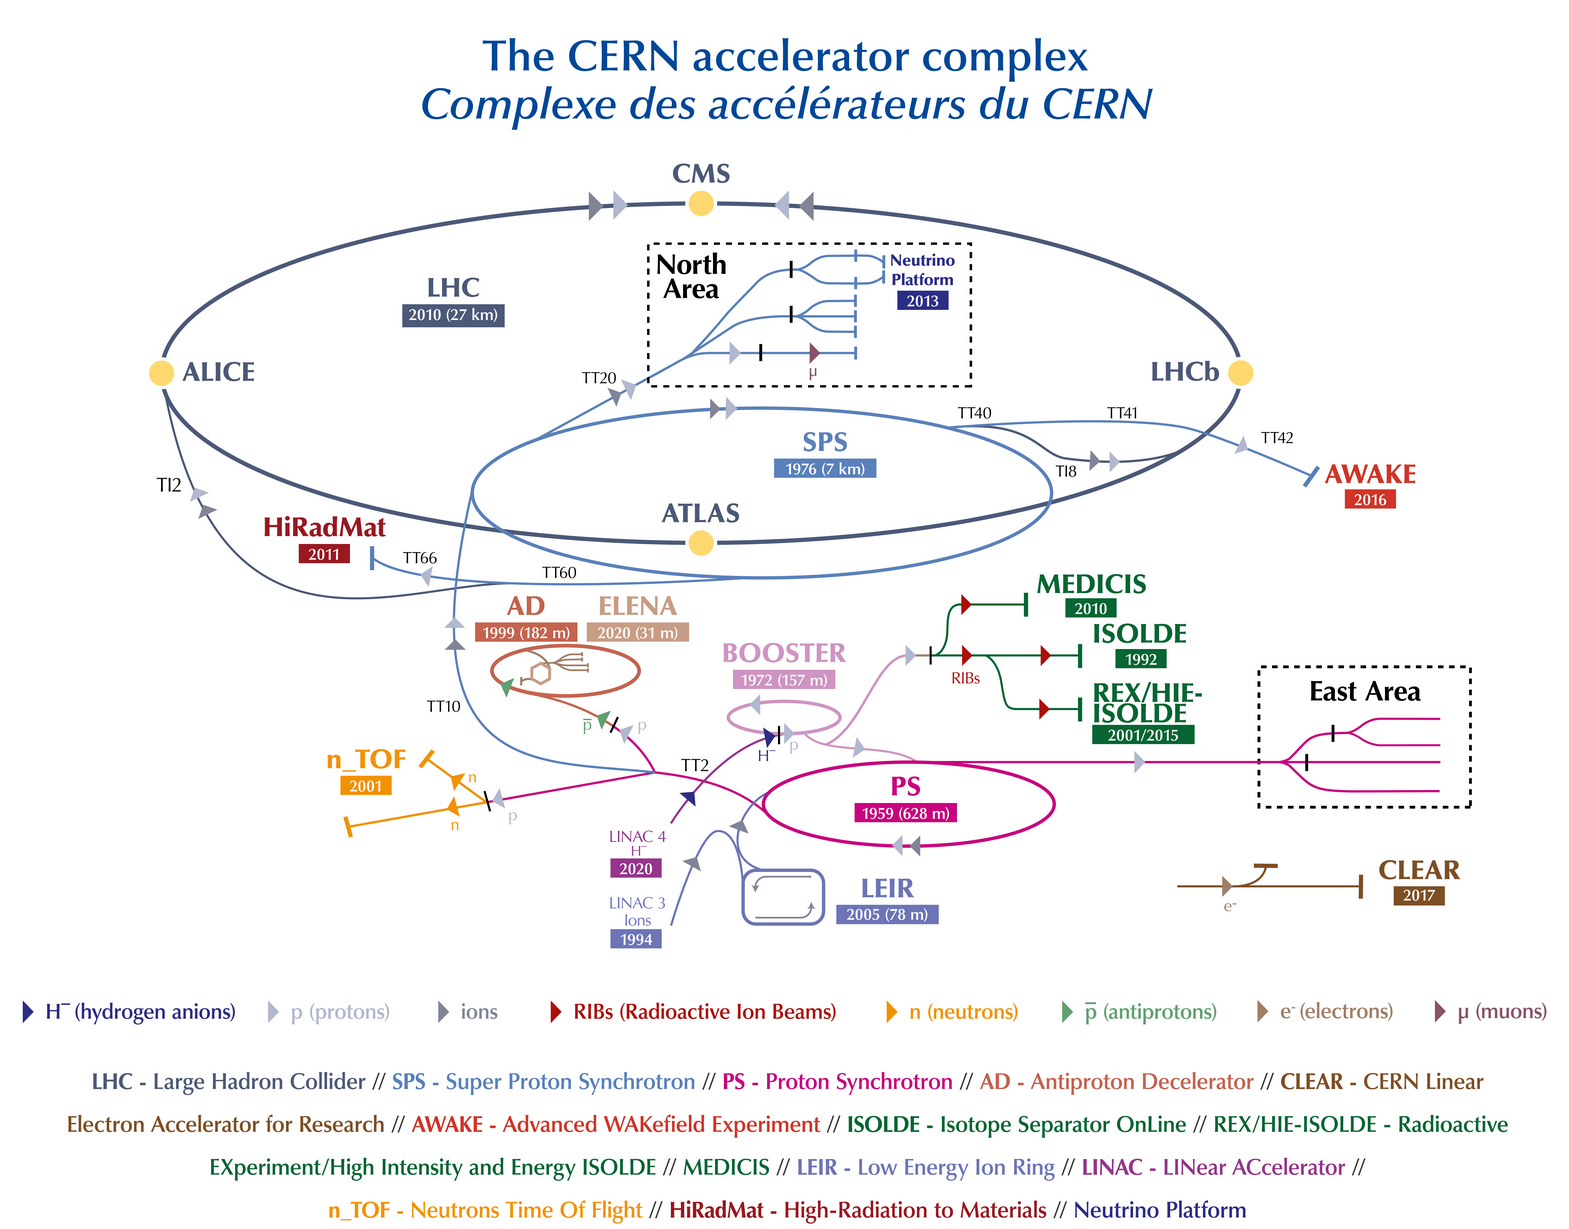
\includegraphics[width=0.99\textwidth]{Figures/cern_atlas/complex.png}
    \caption{The layout of the CERN accelerator complex as of 2022~\cite{CERNAC}.}
    \label{fig:cern_accelerator_complex}
\end{figure}

\subsection{Coordinate Systems}

In collider experiments, the typical coordinate system places the origin at the nominal IP, which, for hermetic detectors like ATLAS, ALICE, and CMS, is at the centre of the detector.
The coordinate systems used by these experiments are right-handed, as shown in \Cref{fig:atlas_coordinate_system}, with the $z$-axis points along the beamline, the $y$-axis pointing upwards, and the $x$-axis pointing towards the centre of the LHC ring.
The transverse plane is defined as the plane perpendicular to the beam axis and is spanned by the $x$ and $y$ coordinates.

A polar representation is also often used, where the azimuthal angle $\phi$ is measured in the transverse plane from the $x$-axis, and the polar angle $\theta$ is measured from the $z$-axis.
The polar angle is frequently replaced with pseudorapidity $\eta$, defined as
\begin{equation}
    \eta = -\ln \left( \tan \left( \frac{\theta}{2} \right) \right).
\end{equation}
Differences in pseudorapidity are Lorentz invariant under boosts in the direction of the beamline, making it a useful quantity for describing the products of high-energy collisions.

Angular distances between objects are often measured in $\Delta R = \sqrt{(\Delta \eta)^2 + (\Delta \phi)^2}$, where $\Delta \eta$ and $\Delta \phi$ are the differences in pseudorapidity and azimuthal angle.
For collision products, a key observable is a transverse momentum $\pt=\sqrt{p_x^2 + p_y^2}$, where $p_x$ and $p_y$ are the components of the momentum in the transverse plane.

\begin{figure}
    \centering
    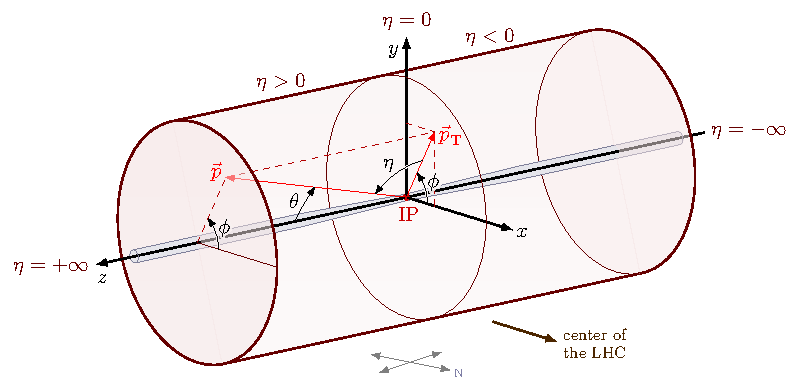
\includegraphics[width=0.6\textwidth]{Feynman/coordinate.pdf}
    \caption{The right-handed coordinate system used by the ATLAS experiment.}
    \label{fig:atlas_coordinate_system}
\end{figure}

\subsection{Cross-Section and Luminosity}

The cross-section, denoted by $\sigma$, indicates the likelihood of an interaction between two colliding particles.
Calculating the cross-section involves quantum mechanical transition matrix elements and phase space integrals, and it can be likened to the effective cross-sectional area of the particles participating in the interaction.
It is typically expressed in units of femtobarns (fb), where $1~\fb = 10^{-28}\unit{\meter^2}$.

The total number of interactions $N$ depends on the cross-section of the process $\sigma$ and the integrated luminosity $L_{\text{int}}$ by the formula,
\begin{equation}
    N = \sigma L_{\text{int}} = \sigma \int \mathcal{L}(t) dt,
\end{equation}
where $\mathcal{L}(t)$ is the instantaneous luminosity.
This measures how tightly packed colliding particles are in a unit of space and time and is
Integrated luminosity has units of inverse area and is typically expressed in inverse femtobarns ($\ifb$).
For two colliding beams with Gaussian densities, the instantaneous luminosity is given by
\begin{equation}
    \mathcal{L}(t) = \frac{N_1 N_2 f}{4 \pi \sigma_x \sigma_y} S(\theta_c),
\end{equation}
where $N_1$ and $N_2$ are the number of particles in each beam, $f$ is the frequency of bunch crossings, $\sigma_x$ and $\sigma_y$ are the root-mean-square beam widths in the $x$ and $y$ directions, and $S(\theta_c)$ is the geometric reduction factor due to the crossing angle $\theta_c$.
This last factor exists because the beams do not collide head-on, as this would result in multiple collision points, so they are crossed at a finite angle $\theta_c$.
This reduces the overlap of the beams when they pass through one another, reducing the effective luminosity.
For the $pp$ collisions at the LHC, $S(\theta_c)$ is measured to be approximately $0.61$.
Even with this finite angle, long-range beam-beam interactions can still occur and must be accounted for.

The LHC was designed to deliver $\mathcal{L}(t) = 10^{34}~\unit{\centi\meter^{-2}\second^{-1}}$ at the IPs of ATLAS and CMS.
However, this has not been constant over the years, and each experiment independently measures the luminosity using well-understood processes.
The total integrated luminosity delivered by the LHC and recorded by ATLAS is shown in \Cref{fig:luminosity}.
The LHC's instantaneous luminosity has increased with each run and this is particularly beneficial for measurements on rare events where the uncertainty is statistically limited.

\begin{figure}
    \centering
    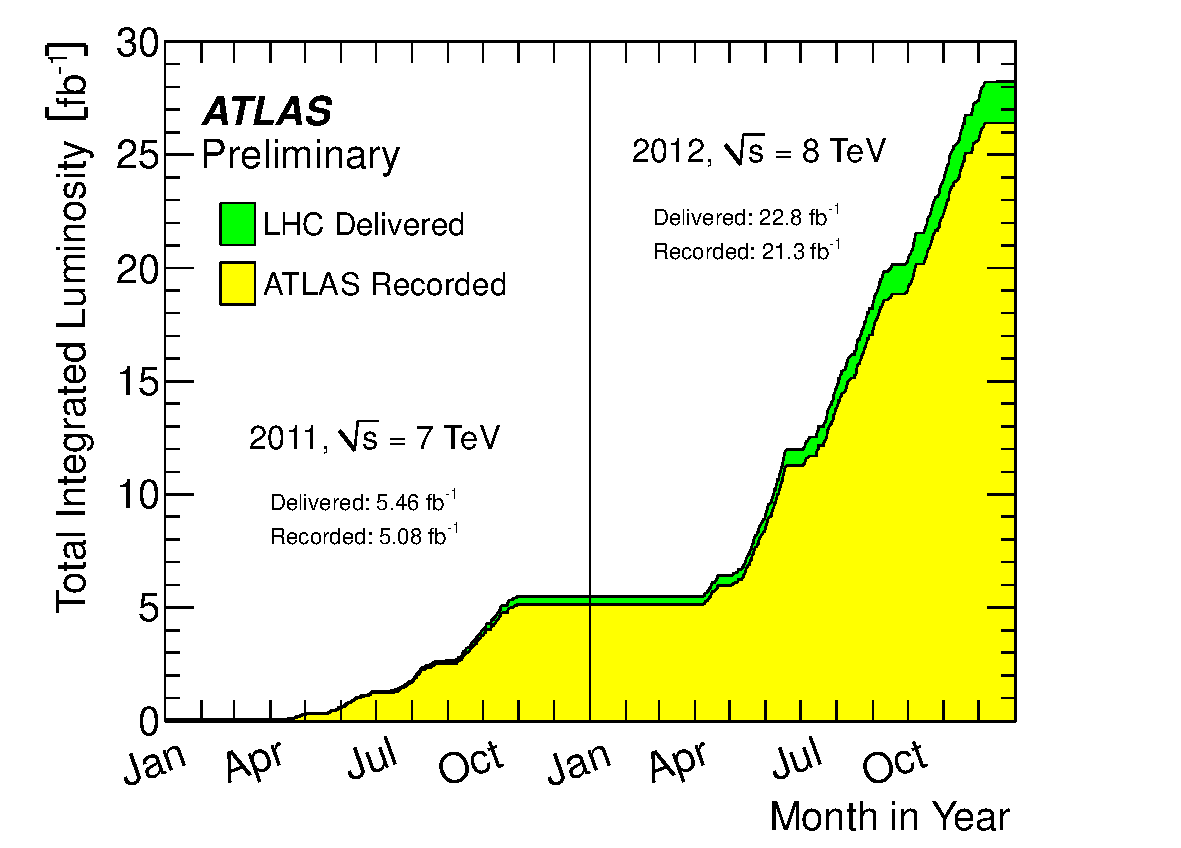
\includegraphics[width=0.32\textwidth]{Figures/cern_atlas/lumi1.pdf}
    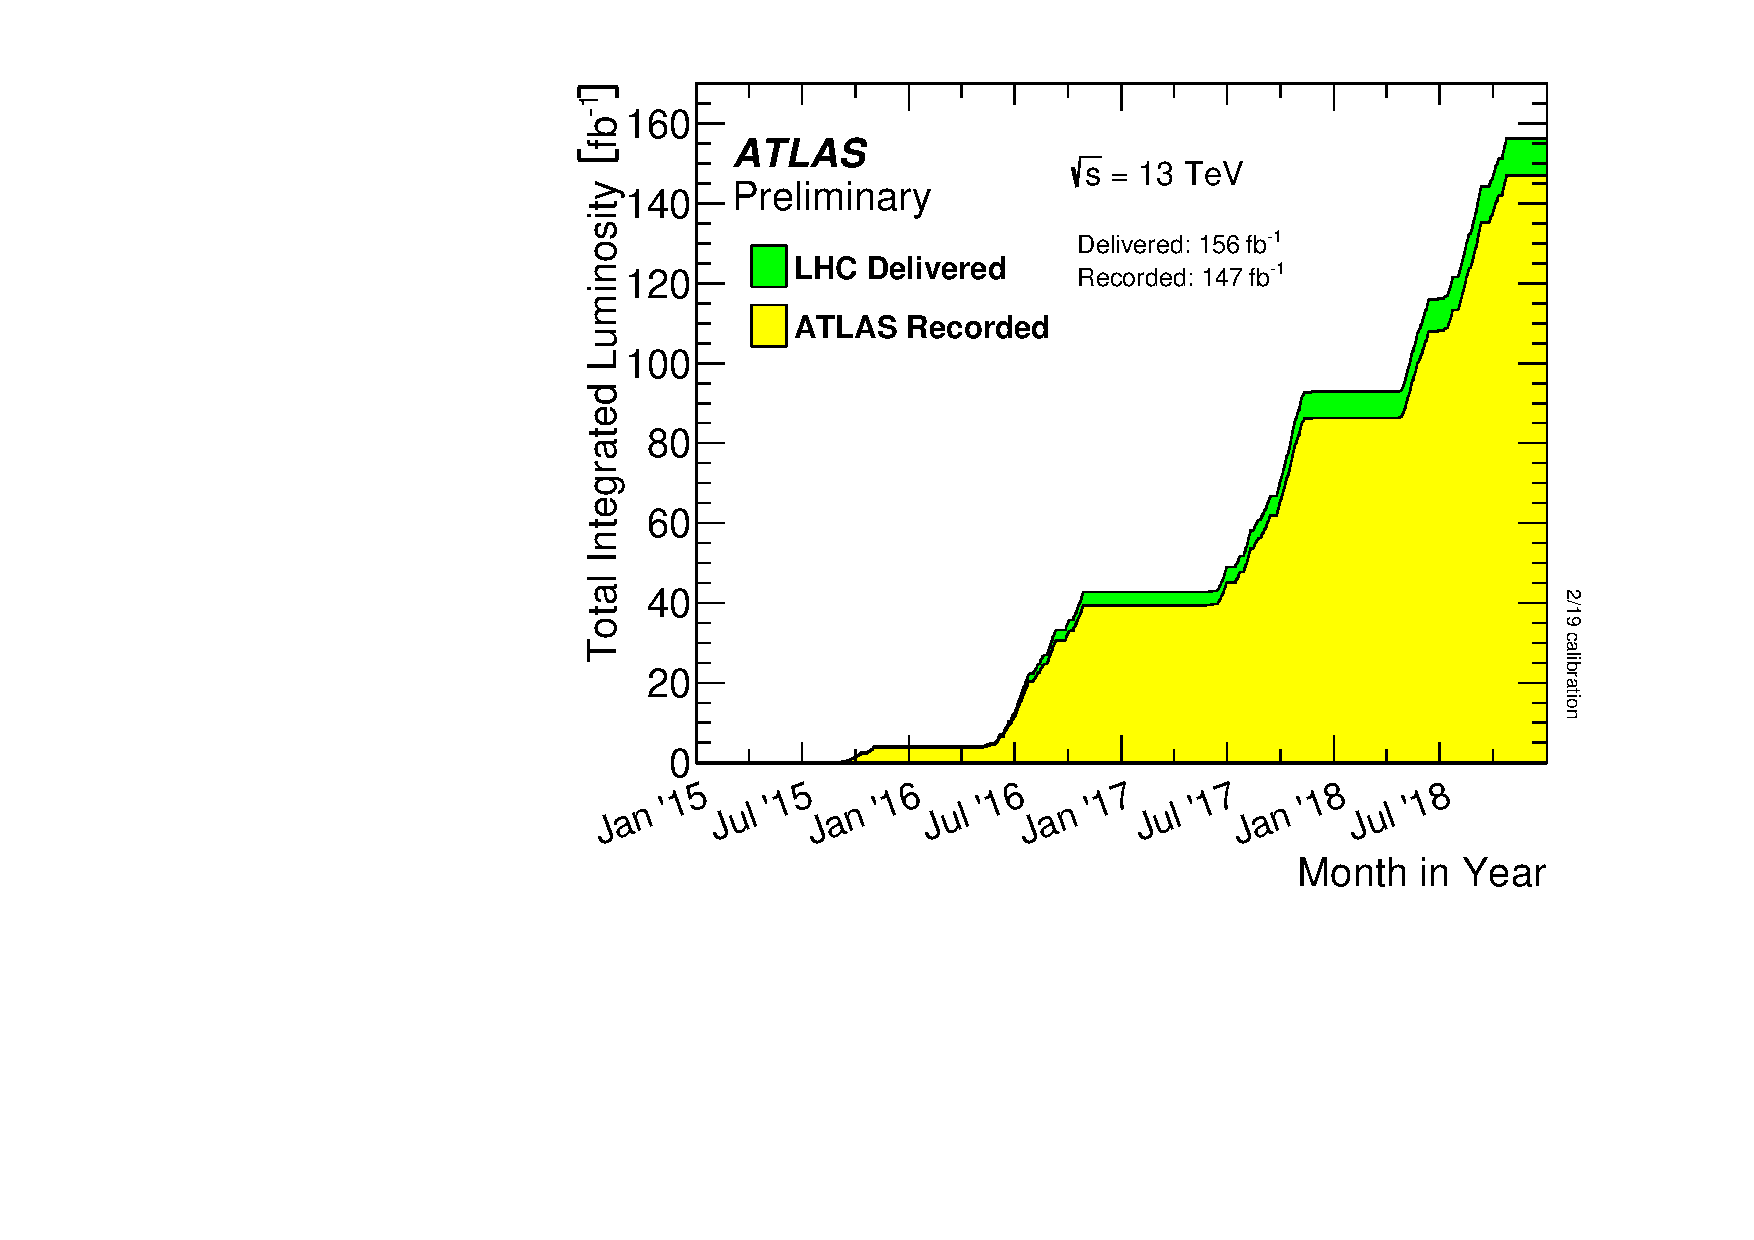
\includegraphics[width=0.32\textwidth]{Figures/cern_atlas/lumi2.pdf}
    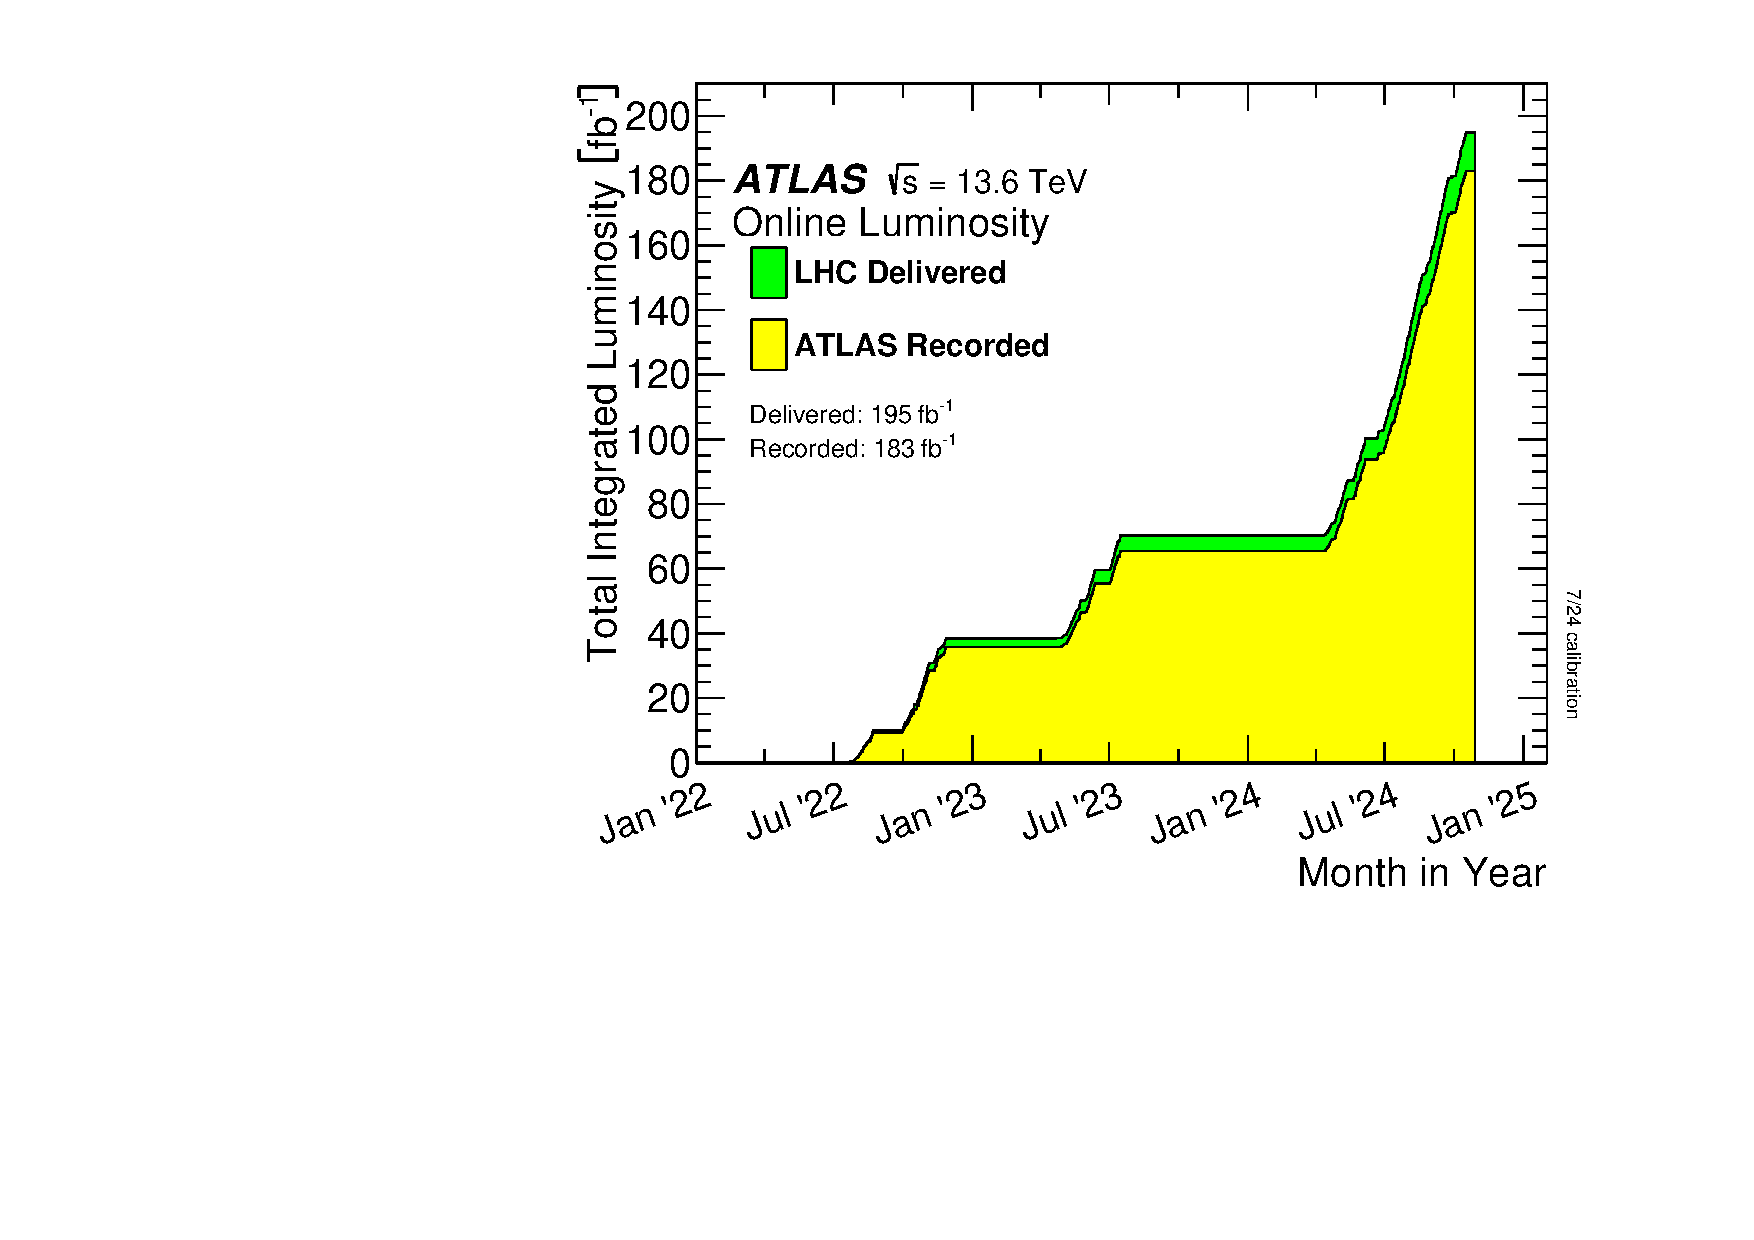
\includegraphics[width=0.32\textwidth]{Figures/cern_atlas/lumi3.pdf}
    \caption{The total integrated luminosity delivered by the LHC and recorded by the ATLAS experiment for Run 1 (left)~\cite{run1data}, Run 2 (middle)~\cite{run2data}, and Run 3 (right)~\cite{run3data}.}
    \label{fig:luminosity}
\end{figure}

\subsection{LHC Runs}

The LHC operates on multi-year runs -- the first began in 2010.
In between each run is a period of \textit{long-shutdown}, allowing for maintenance and upgrades to both the accelerator and the experiments.
The various run properties are shown in \Cref{tab:lhc_runs}.
Due to an electrical fault damaging many of the superconducting magnets in 2008, Run 1 was much delayed and operated at a reduced $\sqrt{s}=7~\TeV$ using a sparse bunch structure, only colliding at $20~\MHz$.
In 2012, the energy was increased to $\sqrt{s}=8~\TeV$.
The total delivered luminosity of the run was $28.4~\ifb$.
Run 2 spanned from 2015 to 2018, with an increased energy of $\sqrt{s}=13~\TeV$, a bunch crossing rate of up to $40~\MHz$, and a total integrated luminosity of $156~\ifb$.
Run 3 began in 2022 and is expected to continue until 2026 and has already surpassed Run 2 with $195~\ifb$ of data delivered~\cite{run3data}.

\begin{table}[h!]
    \centering
    \caption{Overview of the different LHC runs~\cite{LHCRun2,LHCRun3,run1data, run2data, run3data}. Values for Run 3 are preliminary as data is still being collected.}
    \label{tab:lhc_runs}
    \resizebox{\textwidth}{!}{
        \begin{tabular}{lcccccc}
            \toprule
                              & $\sqrt{s}~[\TeV]$ & $\mathcal{L}_\text{int}~[\ifb]$ & Protons per bunch     & Bunch spacing $[\ns]$ & \avemu \\
            \midrule
            Run 1 (2010-2011) & 7                 & 5.5                             & $1.45 \times 10^{11}$ & 50                    & 10     \\
            Run 1 (2012)      & 8                 & 22.8                            & $1.6 \times 10^{11}$  & 50                    & 21     \\
            Run 2 (2015-2028) & 13                & 156                             & $1.25 \times 10^{11}$ & 25                    & 34     \\
            Run 3 (2022-)     & 13.6              & 195                             & $1.8 \times 10^{11}$  & 25                    & 50     \\
            \bottomrule
        \end{tabular}
    }
\end{table}

\subsection{Pileup}

The increase in luminosity between Run 1 and Run 3 was in part achieved by raising the number of protons per bunch.
This in turn leads to more particle interactions per bunch crossing.
One of the undesirable effects of this is the large amount of overlapping signals in the detector which can degrade the resolution and efficiency of reconstruction algorithms.

Each bunch crossing in the collider generates a distinct collision event for the experiments.
As illustrated in \Cref{fig:pileup}, the average number of interactions per crossing has increased with each LHC run.
Typically, only one of the $pp$ interactions, known as the hard scatter, is of primary interest.
The remaining interactions, referred to as ``soft scatters'', are low-energy events collectively known as in-time pileup.
Detector materials have a response and reset time, which can lead to residual signals from previous crossing being rerecorded.
This is known as out-of-time pileup.
Filtering out signals from all pileup sources is crucial for accurate data analysis and poses a significant challenge as the LHC's luminosity increases.

\begin{figure}
    \centering
    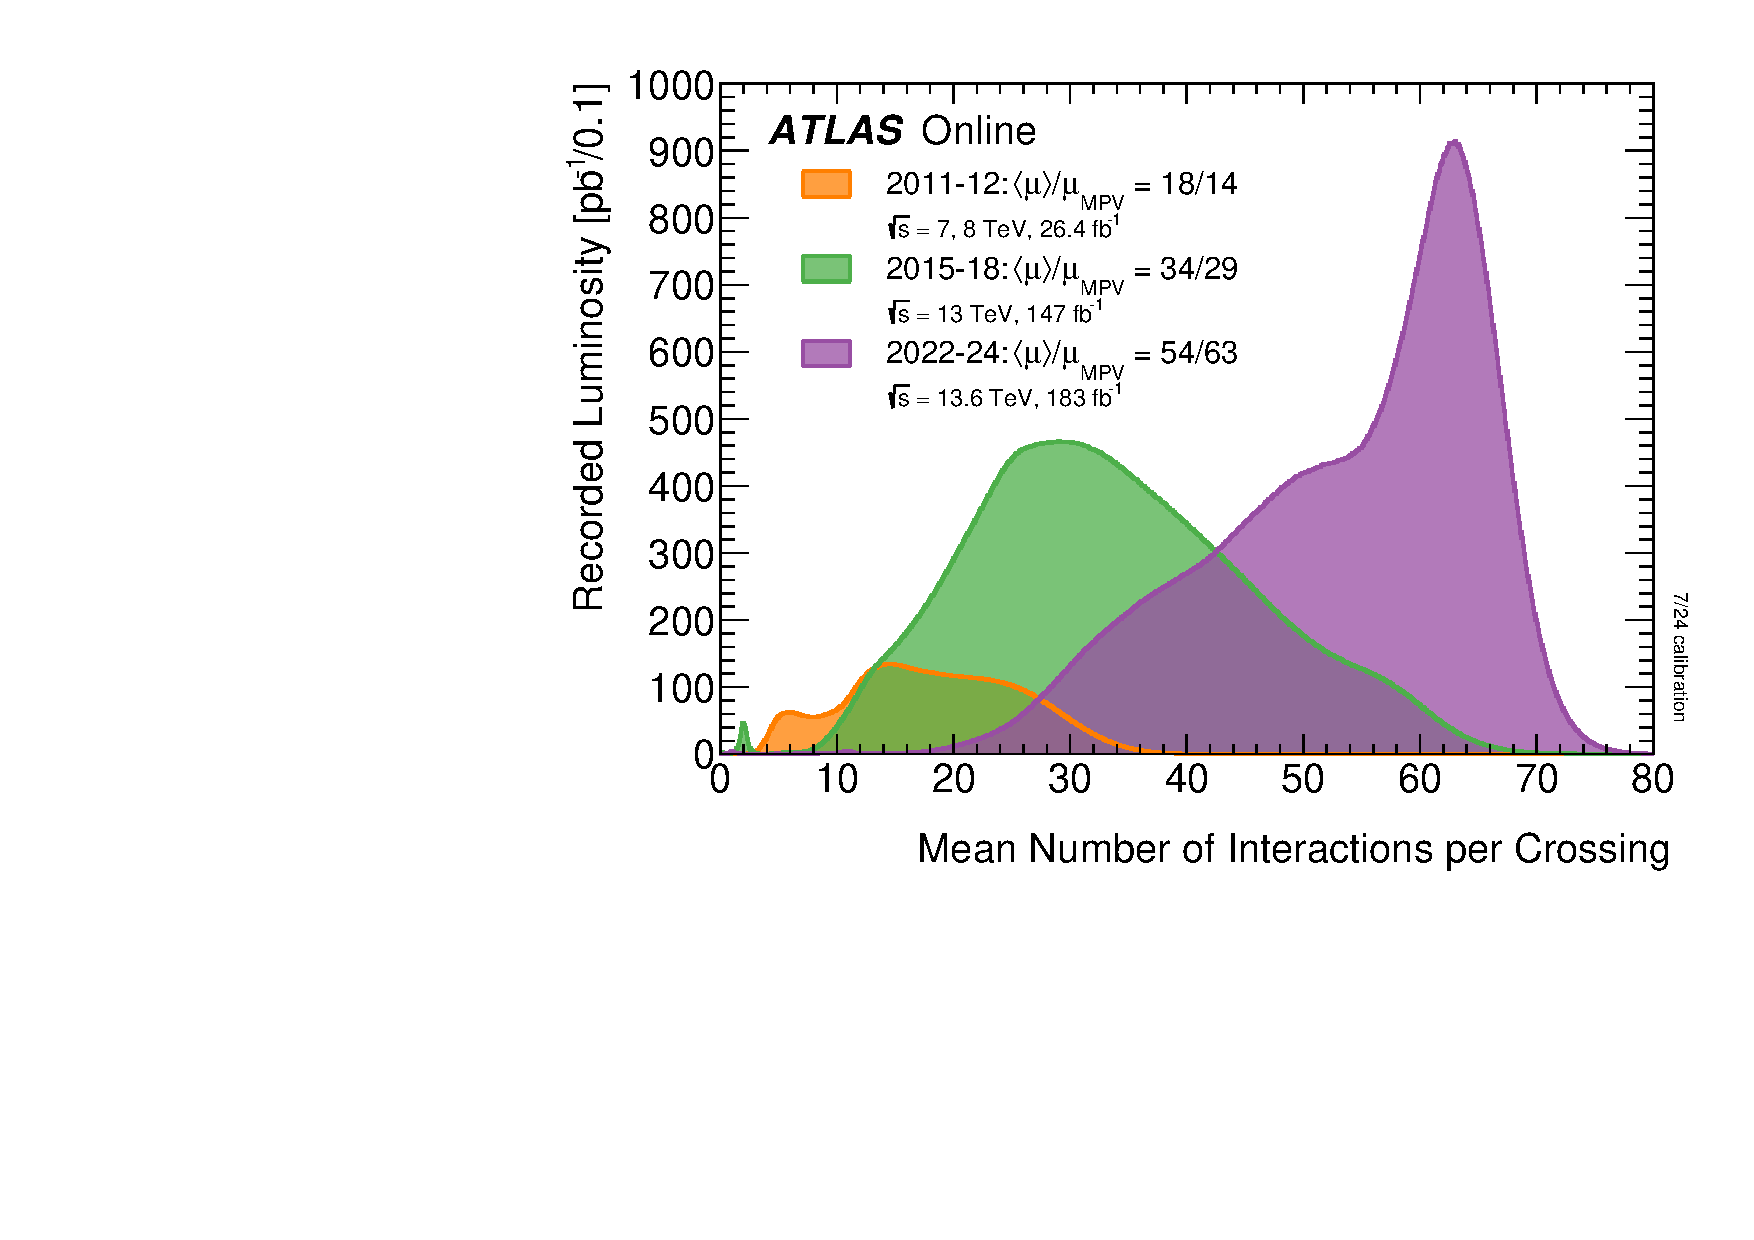
\includegraphics[width=0.6\textwidth]{Figures/cern_atlas/mu_run123.pdf}
    \caption{The distribution of the number of interactions per bunch crossing over the three LHC runs as measured by the ATLAS experiment~\cite{run3data}.}
    \label{fig:pileup}
\end{figure}

\section{The ATLAS Experiment}

The ATLAS experiment~\cite{ATLAS, ATLASRun3} is one of the four primary experiments at the LHC\@.
It is the largest particle detector of the four, weighing $7000$ tonnes and measuring $44$ m long and $25$ m in diameter.
Equipped with multiple sub-detectors, it is a general-purpose detector designed to capture various outgoing products from the $pp$ collisions and explore a wide range of physics phenomena.
The ATLAS detector is shown in \Cref{fig:atlas_detector}.

The detector is hermetic, meaning it covers nearly the entire solid angle of $4\pi$.
It is arranged in concentric cylindrical-like layers around the IP\@.
Each layer contains a barrel region, which wraps around the beamline, and end-cap regions, which cover the flat edges of the cylinder on either side.

This section focusses on the tracking systems of the ATLAS detector, which provide precise position and momentum measurements of charged particles.

\begin{figure}[htb]
    \centering
    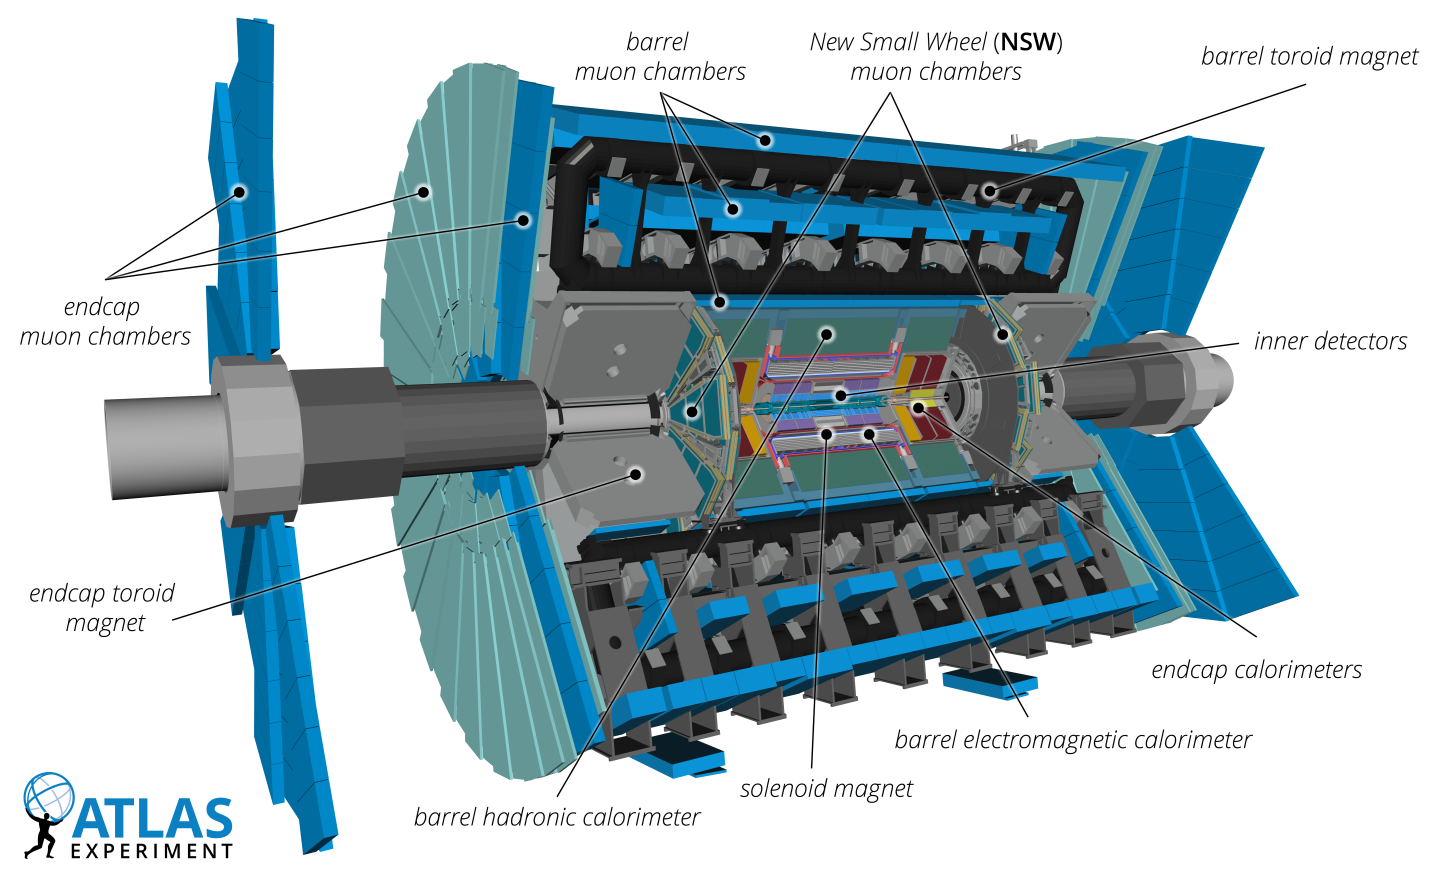
\includegraphics[width=0.99\textwidth]{Figures/cern_atlas/ATLAS.png}
    \caption{The ATLAS detector at the LHC\@. Image taken from Ref.~\cite{ATLASRun3}.}
    \label{fig:atlas_detector}
\end{figure}

\subsection{Inner Detector}

The Inner Detector (ID) is the innermost sub-detector of ATLAS and is shown in \Cref{fig:atlas_inner_detector}.
It comprises three sub-detectors: the Pixel Detector, the Semi-Conductor Tracker (SCT), and the Transition Radiation Tracker (TRT).
It is designed to capture charged particle signals with a pseudorapidity $|\eta| < 2.5$.
These signals are clustered into points in space where the particles have ionized the detector material.
These points can be used to reconstruct the charged particle's trajectory, or \textit{track}, as it propagates from the centre of the detector.

The ID is immersed in a $2~\tesla$ axial magnetic field generated by a 5.8 m long superconducting solenoid magnet containing over $9\km$ of NbTi wire.
The magnetic field causes the particles to bend in a plane perpendicular to the beamline, tracing a helical path whose curvature is proportional to $q/p$, where $q$ is the charge of the particle and $p$ is the magnitude of its momentum.

A fully reconstructed track is characterized by five parameters, which are shown in \Cref{fig:track_parameters}.
These include the charge-to-momentum ratio $q/p$, the azimuthal angle $\phi$, the polar angle $\theta$, the longitudinal impact parameter  $z_0$, and transverse impact parameter $d_0$.
The impact parameters represent the distance between the track and the IP, measured at the point of closest approach between the track and the beamline.
The relative $\pt$ resolution of the ID is described as,
\begin{equation}
    \sigma(\frac{1}{\pt}) = 0.36 \oplus \frac{13}{\pt \sin(\theta)}~\TeV
\end{equation}
where $\oplus$ denotes a sum in quadrature.

\begin{figure}[htb]
    \centering
    \includegraphics[width=0.6\textwidth]{Figures/cern_atlas/Track.png}
    \caption{The main parameters of a reconstructed track in the ATLAS Inner Detector. Image taken from Ref.~\cite{ATLASTrackingSoftware}.}
    \label{fig:track_parameters}
\end{figure}

\begin{figure}[htb]
    \centering
    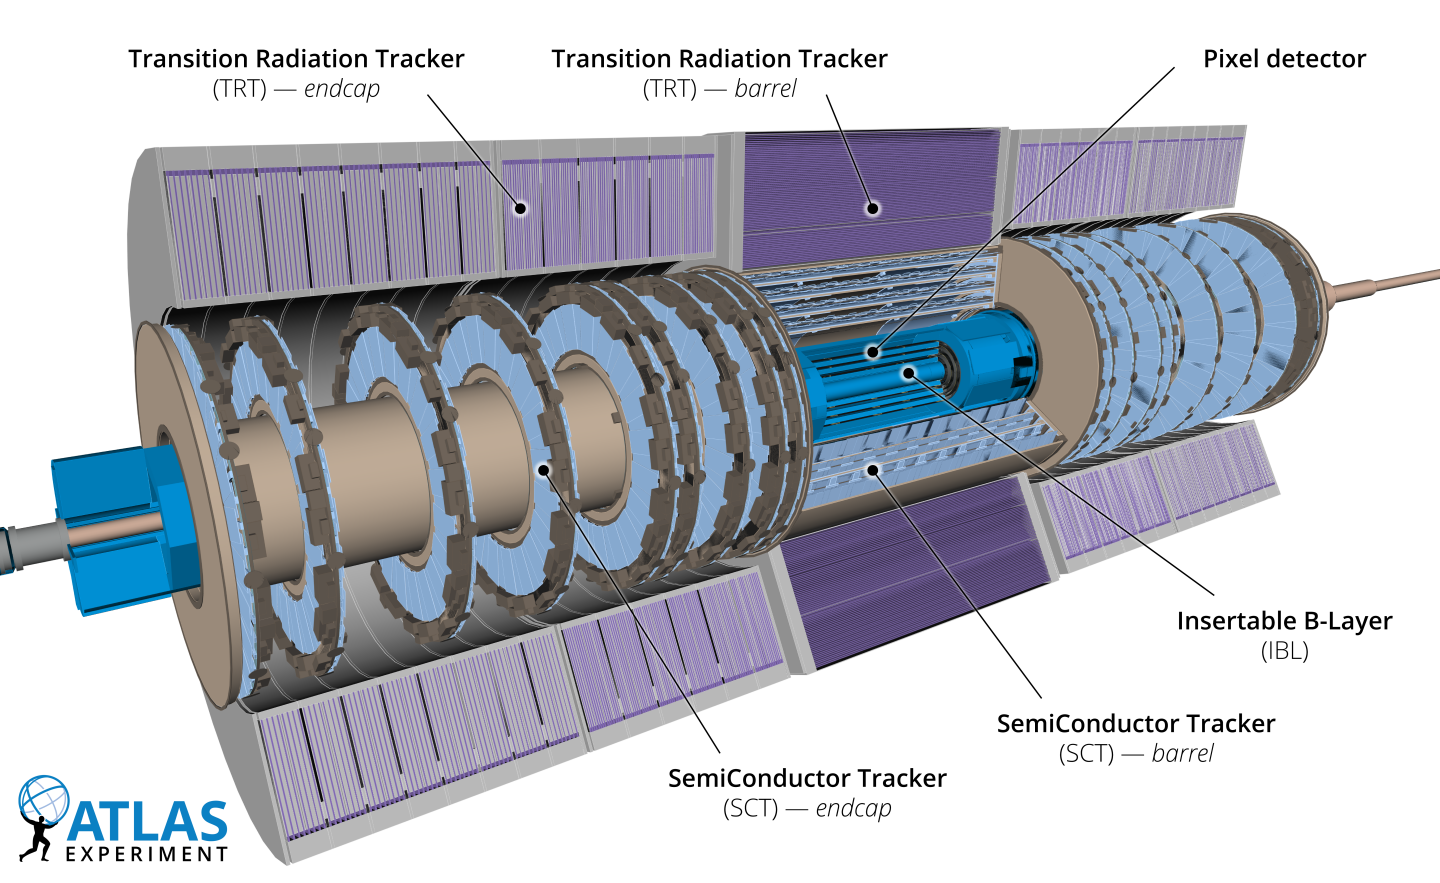
\includegraphics[width=0.59\textwidth]{Figures/cern_atlas/BetterID.png}
    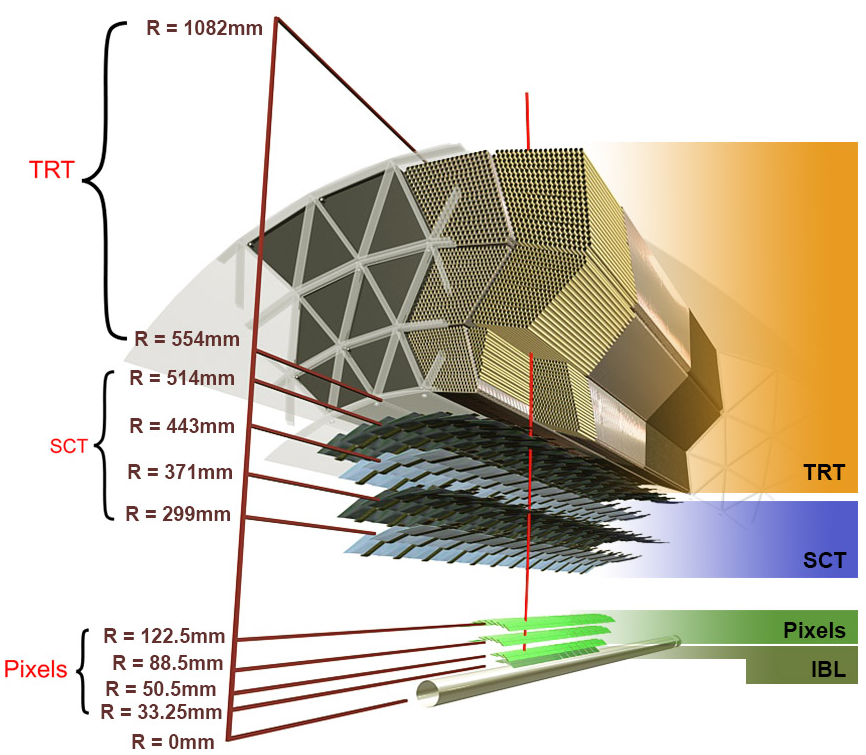
\includegraphics[width=0.39\textwidth]{Figures/cern_atlas/IDCut.png}
    \caption{Schematic of the full ATLAS Inner Detector (left) and a cross-section of the barrel region (right). Images taken from Refs.~\cite{ATLASRun3,IBLPhotos}.}
    \label{fig:atlas_inner_detector}

\end{figure}

\subsubsection{Pixel Detector}

The high-granularity silicon pixel detector~\cite{ATLASPixel} covers the innermost region of the ID.
It measures 1.4 m long and is fully contained in a diameter of 0.5 m.
High granularity is required at this scale to resolve the numerous tracks that pass through it.
Individual silicon pixels are about $50~\um$ wide in the transverse direction and about $400~\um$ long in the longitudinal direction.

Each pixel has a slight potential difference applied across it.
Ionizing radiation left by a traversing charged particle generates electron-hole pairs that drift and are collected at the p-n junctions, providing a signal.
The pixel detector has 1744 modules, each containing around 46k pixels, resulting in 80M readout channels.
These are arranged in three barrel layers placed at a radius of $50.5~\mm$, $88.5~\mm$, and $122.5~\mm$ from the beamline, with four end-cap disks on each side.

Between Run 1 and 2, an additional layer was added at a radius of $33~\mm$ to the beamline, known as the Insertable B-Layer (IBL)~\cite{ATLASIBL}.
Pixels in the IBL measure $50~\um$ in the transverse direction and $250~\um$ in the longitudinal direction.
This layer improved the $\pt$ resolution of the detector by close to 30\% for low $\pt$ tracks.
Furthermore, the enhanced $z$-resolution improved impact parameter resolution and cluster separation, allowing for better reconstruction of primary and secondary vertices.

\subsubsection{Semiconductor Tracker}

The Semiconductor Tracker (SCT)~\cite{ATLASSCT} surrounds the Pixel Detector, occupying the region between $299~\mm$ and $514~\mm$ from the beamline.
It comprises four concentric barrel layers with nine disks at each end-cap covering the region $|\eta| < 2.5$.
Like the pixel detector, the SCT is composed of silicon readout channels. Unlike the pixels, each microstrip measures $20~\um \times 12~\cm$ and thus only has high granularity in a single direction, oriented to the transverse momentum.
To improve longitudinal resolution, each SCT layer includes two back-to-back microstrip layers, rotated by $40 \unit{\milli\radian}$ relative to each other.
The SCT in total has around 6.3M readout channels.

\subsubsection{TRT}

The outermost sub-detector of the ID is the Transition Radiation Tracker (TRT)~\cite{ATLASTRT}.
It is a straw-tube tracker that aids in the momentum measurement and provides information for particle identification for tracks within $|\eta| < 2.0$.
The TRT provides the most hits per track of the three sub-detectors -- approximately 35 hits on average.
At a greater distance from the beamline, it also does not require such fine spatial resolution as the silicon detectors to provide an accurate measurement of the track kinematics.

The TRT comprises approximately 300k thin-walled drift tubes, each $4~\mm$ in diameter.
The barrel region contains 50k tubes, each $144~\cm$ long, while the end caps contain 250k tubes, each $37~\cm$ long.
A potential difference exists between the tube walls and an axial wire.
When a charged particle intersects the tube, it ionizes the predominantly argon gas inside, and the resulting electrons drift towards the wire, providing the signal.
There is no information on where the ionization occurred along the length of the tube.
Thus, resolution for the barrel region is defined in the $r-\phi$ plane, while the end-cap resolution is defined in the $r-z$ plane.
A polymer foil is placed between the tubes to generate transition radiation, the pattern of which allows discriminating between electrons and pions.

\subsection{Calorimeters}

ATLAS has three calorimeter systems outside the central solenoid magnet, which measure the energy of particles produced by the collisions.
Each calorimeter is designed with alternating layers of absorber and active materials.
Particles interact with the absorbers, lose energy, and produce showers of secondary particles that ionize the active material, which can be converted into a measurable signal.
These layers are typically arranged in an accordion-like structure to ensure homogenous coverage.
Different absorber materials are used to optimize the containment of the showers belonging to different particle types.

The Electromagnetic Calorimeter (ECal) is specialized for measuring the energy of electrons and photons.
Surrounding this is the Hadronic Calorimeter (HCal), which is designed to measure the energies of hadrons.
These subsystems cover the region $|\eta| < 3.2$.
In addition, there is also the forward calorimeter subsystem, which measures the energy of particles in the range $3.2 < |\eta| < 4.9$.
However, information from this subsystem is not used in this thesis, and it is omitted from the following descriptions.
A schematic of the calorimeter system is shown in \Cref{fig:atlas_calorimeters}.

\begin{figure}[htb]
    \centering
    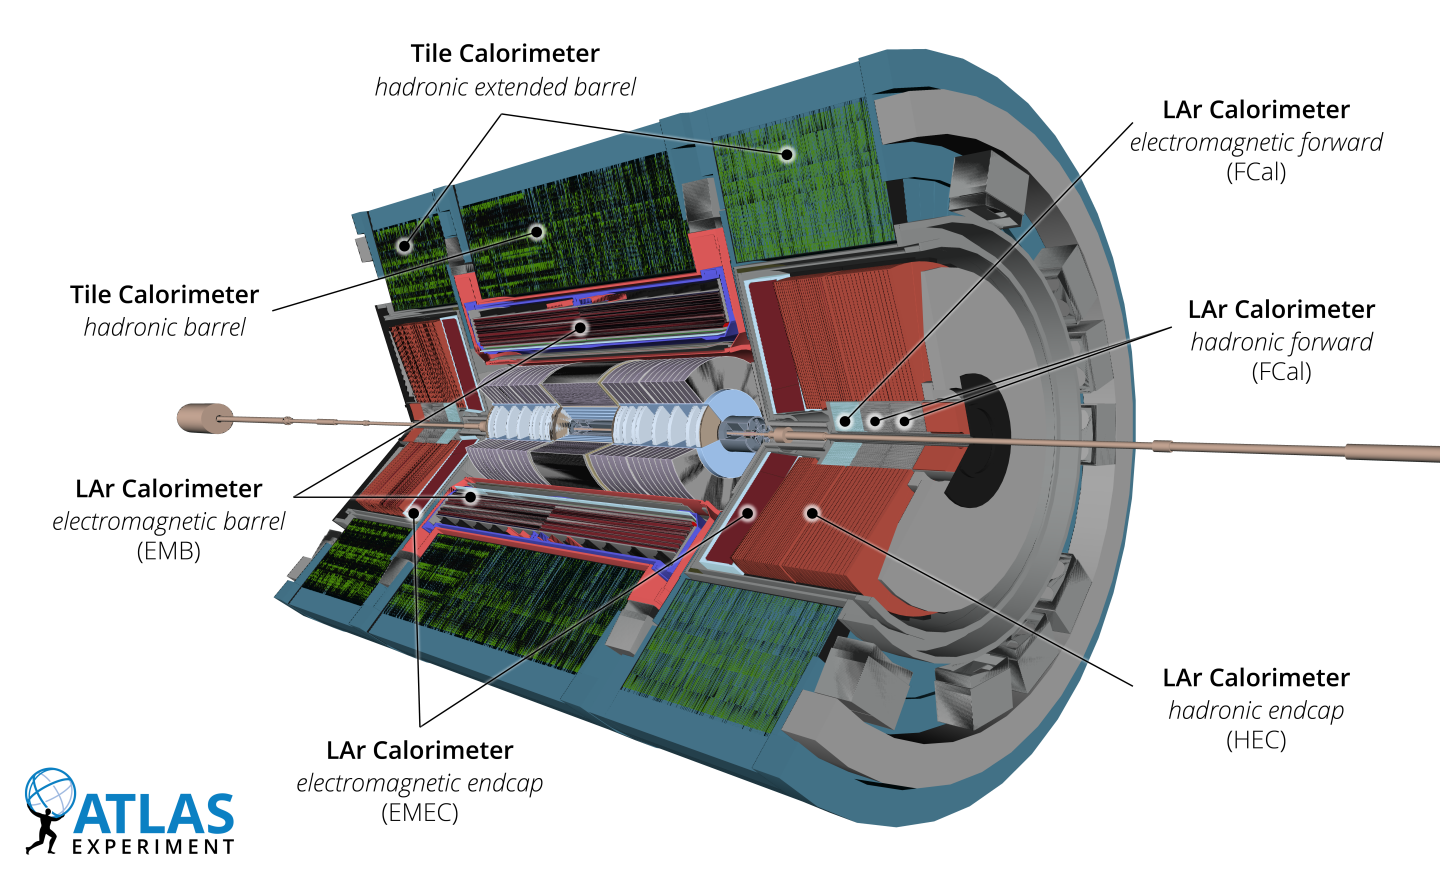
\includegraphics[width=0.99\textwidth]{Figures/cern_atlas/Calos.png}
    \caption{Schematic of the ATLAS calorimeter systems. Image taken from Ref.~\cite{ATLASRun3}.}
    \label{fig:atlas_calorimeters}
\end{figure}

\subsubsection{Electromagnetic Calorimeter}

The ECal~\cite{ATLASECal} is a high granularity calorimeter which uses liquid argon as the active material and lead as the absorber.
To keep the argon in a liquid state, the ECal is cooled to $-185~\unit{\degree C}$.
These materials are chosen to optimize the containment of electromagnetic showers produced by electrons and photons, via pair production and bremsstrahlung radiation, while minimising the energy loss of heavier particles.
The barrel ECal covers the range $|\eta| < 1.475$ and is split into three layers, decreasing in granularity with distance from the beamline.
The inner layer allows for more precise shower measurements which assists in the identification of pions.
The Liquid Argon Electromagnetic Enc-Cape (EMEC) and covers the range $1.375 < |\eta| < 3.2$.
Unlike the ID, the ECal resolution increases with incident particle energy.

\subsubsection{Hadronic Calorimeter}

The HCal (or Tile Calorimeter)~\cite{ATLASHCal} surrounds the ECal and is engineered to accurately measure the energy of hadrons.
It uses steel as the absorber and scintillating tiles as the active material made from polystyrene.
The hadrons are contained by losing energy through inelastic nuclear interactions with the steel, producing a shower of electrons and photons which are detected by the tiles.
In the forward regions of the calorimeter, $1.5 < |\eta| < 3.2$, a copper/LAr combination is used.
The granularity and energy resolution of the HCal are lower than the ECal.

\subsection{Muon Spectrometer}

Other than neutrinos, which traverse the entire detector without interacting, muons are the only particles that easily penetrate through the calorimeters, incurring minimal energy loss.
Though they leave tracks in the ID, the Muon Spectrometer (MS)~\cite{ATLASMuon,ATLASRun3} provides triggering information, identification, and extra momentum measurements for muons.
The MS is the outermost sub-detector of ATLAS and is shown in \Cref{fig:atlas_muon_spectrometer}.
Its systems are arranged in three barrel layers covering $|\eta| < 1.2$ and several end-cap layers or wheels covering $1 < |\eta| < 2.7$.
The wheels are placed on either side of the detector at a distance of $7.4$~m, $14$~m, and $21.5$~m from the IP.

Monitored Drift Tubes are the spectrometer's primary tracking component and are similar in principle to the straw tubes in the TRT\@.
More than 380k aluminium tubes, each with a diameter of $30$~mm and primarily filled with argon gas, are organized into three barrel layers and four end-cap disks.
In addition, Cathode Strip Chambers are used in inner layers of the end-cap to cope with the higher particle flux.
These are multi-wire proportional chambers built into strips.

Three large air-core toroidal magnets generate the magnetic field in the MS\@, one in the barrel region and one in each end-cap regions.
Each magnet has eight coils and deflects the muons, allowing for the measurement of their momentum.

\begin{figure}[htb]
    \centering
    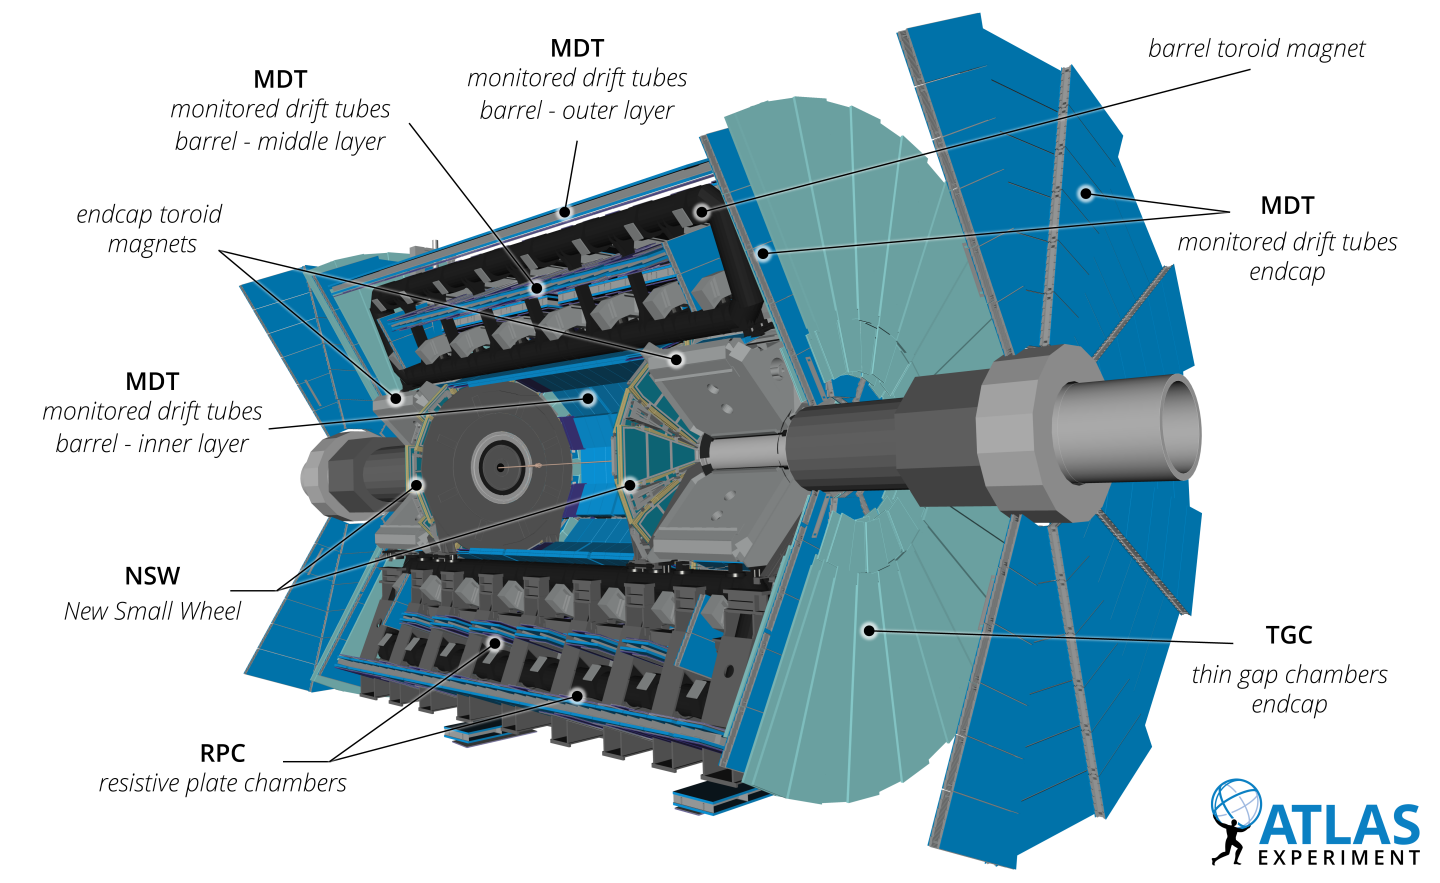
\includegraphics[width=0.99\textwidth]{Figures/cern_atlas/MS.png}
    \caption{Schematic of the ATLAS Muon Spectrometer. Image taken from Ref.~\cite{ATLASRun3}.}
    \label{fig:atlas_muon_spectrometer}
\end{figure}

\section{Reconstruction}
\label{sec:event_reconstruction}

Reconstruction is the process of converting the raw detector signals into collections of defined physical objects to better understand the collision events.
This process is performed offline, after the data has been recorded and stored, and uses information from all sub-detectors.

Additionally, the components of this thesis which utilized official ATLAS simulation and software, covered in \Cref{ch:spice}, are limited to tracks and jets.
Therefore, the information provided here is focused on these topics only.

This section describes the basics of track, vertex, and jet reconstruction at ATLAS, as well as several approaches to jet tagging.

\subsection{Tracks}

Track reconstruction involves collecting hits registered by the ID and organizing them into distinct tracks, which are most likely produced by individual charged particles.
Tracks are key ingredients in the reconstruction and identification of various physics objects, such as electrons and muons, jets, and the multiple vertices produced in each collision.
A full description of the track reconstruction pipeline used for ATLAS Run 2 data can be found in Ref.~\cite{PerformanceATLASTrack}.
Track reconstruction is performed in numerous stages.
Hits are first clustered into space points, after which iterative track-finding algorithms are used, followed by cleaning and ambiguity resolution.
This process may lead to tracks being mistakenly reconstructed from hits left by multiple particles, or other background sources, and these are referred to as \textit{fake tracks}.

\subsubsection{Clusterization}

A single particle may deposit energy in multiple adjacent pixels or strips in the ID\@.
This is due to the drift of electrons between sensors within the solenoid magnetic field or from the incident angle of the particle.
These hits are first combined into clusters which are then used to form \textit{space points} (SP) defined in three dimensions.
For the SCT, these clusters also combine information from the two back-to-back layers.
Position uncertainties of these points are estimated from cluster sizes and detector geometry.
In dense environments the clustering algorithm may mistakenly merge hits from different particles, leading to a higher rate of fake tracks.

\subsubsection{Track Seeding}

Tracks are \textit{seeded} by grouping triplets of SPs in three sequential layers in either the pixel or SCT subdetectors.
Each of these seeds forms a \textit{track candidate} and are used to determine the first crude estimates of the track parameters, assuming a perfectly uniform magnetic field and helical trajectory.
The only requirement to improve purity is that one additional SP must be found outside the seeding region which compatible with the candidate.

A combinatorial Kalman filter~\cite{ApplicationKalmanFiltering} is employed to iteratively extend this candidate by incorporating additional SPs in the other layers both towards and away from the IP\@.
If multiple compatible space-point extensions are found on the same layer, the filter generates several track candidates for each seed.
At this stage, hits may be shared between multiple candidates, which is intentionally done to maximize the number of possible candidates and thus the efficiency of the algorithm.

The following steps are designed to improve the track quality and remove fake tracks.

\subsubsection{Ambiguity Resolution}

The ambiguity resolver begins by defining a \textit{track score} for each candidate.
This score quantifies the likelihood that each candidate corresponds to a real trajectory.
The score takes into account several factors; the number of SP assigned to the track will increase its score, while the number of holes will decrease it.
Holes are defined as intersections between the reconstructed track and active sensor material where no matching SP is found.
They can be found in data due to inefficiencies in the silicon sensors.
The track score also considers the $\chi^2$ of the track fit.
Tracks with higher \pt also receive a higher score.
The ambiguity resolver then iterates through the list of track candidates in order of decreasing score.

Clusters can overlap naturally in high-density environments.
These are referred to as \textit{merged clusters}.
A neural network\footnote{Neural networks are covered in \Cref{ch:deep_learning}.} estimates the number of particles traversing each cluster and their positions~\cite{NeuralNetworkClustering}.
This information allows the cluster to be split and allocated to the different candidates.
A track can have no more than two shared clusters, and clusters may be shared by no more than two tracks, with preference given to the track with the highest score.
The refined and purified track candidates are then re-fit to obtain the final parameters.
It obtains a new score and is inserted back into the list of candidates.

During this stage, seeds that fail the track-finding process are checked for compatibility with information from the calorimeter.
If a seed is within a region of interest in the calorimeter, the track-finding procedure is repeated, permitting an extra \textit{kink} in the track as this may have been caused by Bremsstrahlung radiation.
This step improves electron reconstruction efficiency.

The ambiguity resolver fully rejects track candidates if they fail to meet the criteria in \Cref{tab:track_criteria}.
If the track is processed twice by the resolver without modification, it is saved to the final collection and all associated hits are removed.

\begin{table}[h!]
    \centering
    \begin{tabular}{ll}
        \toprule
        Parameter           & Selection   \\
        \midrule
        $p_T$               & $> 400$ MeV \\
        $|\eta|$            & $< 2.5$     \\
        $|d_0|$             & $< 3.0$ mm  \\
        $|z_0 \sin \theta|$ & $< 5$ mm    \\
        Shared clusters     & $< 2$       \\
        SCT + Pixel hits    & $\geq 8$    \\
        Pixel holes         & $< 2$       \\
        SCT + Pixel holes   & $< 3$       \\
        \bottomrule
    \end{tabular}
    \caption{Track selection criteria used by the ambiguity resolver.}
    \label{tab:track_criteria}
\end{table}

\subsubsection{TRT Extension}

Finally, information from the TRT is used to extend the tracks.
A similar Kalman filter incorporates TRT hits starting from the predicted intersection between each silicon track and the TRT.
If successful, the TRT hits are added to the track, and the whole track is fitted once more using a global $\chi^2$ fitter.
The inclusion of TRT hits enhances momentum resolution and allows for particle identification.
However, the extension may be rejected if it worsens the $\chi^2$ of the track candidate or if more than 50\% of the TRT hits are tube hits with no leading edge.

\subsection{Vertices}

Vertex reconstruction is the process of identifying the many primary and secondary vertices produced in each collision.
Each vertex is a location in space, constructed from a convergence of fully reconstructed tracks, and indicates the point of origin for multiple charged particles.

Primary vertices are those produced by the many $pp$ collisions during the bunch crossing.
For Runs 1 and 2, primary vertices are reconstructed using the Iterative Vertex Fitter~\cite{ATLASVertex}.
Initially, a seed position for the vertex is chosen based on the mode of the $z$-coordinates of all tracks in the event, measured at their points of closest approach to the beamline.
The vertex position is then iteratively refined, with less compatible tracks being down-weighted in each iteration.
After the final iteration, all tracks with low enough weights are removed from the vertex and used to fit the for the next one.
This process is repeated until no more vertices can be found.
Reconstruction on Run 3 data switched to an Adaptive Multi-Vertex Fitter~\cite{Run3Vertex}.

For each event, the primary vertex with the highest $\Sigma\pt^2$ of all associated tracks is labelled as the \textit{hard scatter vertex}.
It is sometimes ambiguously referred to as \textit{the} primary vertex (PV) while the others are referred to as \textit{pileup} vertices.

Secondary vertices are those produced by the decay of particles originating from the PV.
This secondary decay must take place at a distance sufficiently far away in the transverse plane to be resolved and not mistakenly identified as pileup.
They are typically caused by the decay of long-lived $b$-hadrons or the interaction of particles with the detector material and are thus crucial tools for identifying $b$-jets.
In ATLAS, secondary vertex reconstruction is performed within the context of jet reconstruction using the JetFitter~\cite{JetFitter} or SV1~\cite{SV1} algorithms.

\subsection{Jets}
\label{sec:jets_reconstruction}

As described in \Cref{sec:jets}, jets are an emergent property of QCD\@, which results in a collimated spray of particles stemming from the decay and fragmentation of an initiating color-charged parton.
From a detector perspective, jets result in large localized energy deposits in both calorimeters and many tightly packed tracks in a cone emanating from the PV.
The approximate maximal angular separation of constituents within the jet depends on the mass of the initiating particle and its transverse momentum, with $\Delta R_\text{max} \approx \sfrac{2m}{\pt}$.
Within this region will also include particles emitted from other sources, such as initial state radiation, multiple parton interactions (from the underlying event), or pileup.
Due to the stochastic nature of the showering process, the jet signal can never be perfectly isolated from these backgrounds.
Jet reconstruction is, therefore, a difficult optimization problem.
The goal is to maximally capture the energy of the initiating particle while minimizing the contamination from other sources.
A given jet reconstruction algorithm should capture all hard partons in the event, have an axis parallel to the jet momentum, and accept roughly uniform contamination.

Jet reconstruction in ATLAS is performed using the anti-$k_t$ algorithm~\cite{AntiKt}.
It is a sequential recombination algorithm that iteratively clusters a collection of objects into jets in a manner that is both infrared and collinear safe.
The algorithm is defined by a maximum distance parameter $R$.
The algorithm begins with the hardest, highest \pt, object in the event at index $i$.
During each iteration, the distance $d_{ij}$ is calculated to all other objects $j$ in the event,
\begin{equation}
    d_{ij} = \frac{1}{\max(\pt{_i}^2, \pt{_j}^2)} \frac{\Delta R_{ij}^2}{R^2}.
\end{equation}
If this value is less than $\sfrac{1}{\pt{_i}^2}$, then the objects are combined, and the algorithm proceeds; otherwise, the object at index $i$ is considered a jet and removed from the list.
The algorithm continues until all objects are clustered or declared as jets.

Jets can be clustered using the anti-$k_t$ algorithm with a variety of inputs.
During Run 1, jets were constructed from topo-clusters, topologically connected calorimeter cells~\cite{TopoJets}.
In some analyses, jets are clustered from tracks only~\cite{TrackJets}.
The general approach for Run 2 and 3 data is to include both sets of information using the Particle Flow (PFlow) algorithm~\cite{PFlow}.

\subsubsection{Particle Flow}

The PFlow algorithm is designed to prevent the double-counting of momentum contributions from charged particles that leave both ID tracks and calorimeter energy deposits.
This algorithm iterates through the tracks in descending \pt order, constructing charged PFlow objects.
The algorithm begins by attempting to match the selected track to a topo-cluster in the calorimeter.
Both are then used to compute the expected energy contribution to the cluster by the particle that created the track.
A single particle may deposit energy in multiple topo-clusters, and the algorithm evaluates the probability of this occurring and may include additional topo-clusters if necessary.
The expected energy is then subtracted from the associated topo-clusters, cell-by-cell.
A new track is then selected, and the process is repeated.
If, at any point, the remaining cell energy following the subtraction falls below expected shower fluctuations, it is removed.

Topo-clusters not matched to any tracks are deemed to have been produced from neutral particles and left unmodified.
These, and the remaining clusters after the subtraction step, are used to construct neutral PFlow objects.

The output of the PFlow algorithm is a collection of charged and neutral PFlow objects, each with defined energy and momentum.
Charged PFlow objects not matched to the PV are removed to reduce pileup contamination.
The remaining objects are clustered into jets using the anti-$k_t$ algorithm with $R=0.4$.

\subsubsection{Jet Association}

Once jets are defined, other objects can be associated using a $\Delta R$ matching criterion.
For instance, a jet might be constructed from calorimeter energy deposits, but tracks can still be associated.
The width of the $\Delta R$ association cone typically decreases as with jet \pt.
This track association is beneficial for the ATLAS experiment because it enables using the Jet Vertex Tagger (JVT)~\cite{JVT}.
The JVT leverages the transverse momenta from associated tracks to discriminate against jets originating from pileup interactions.
Furthermore, many of the flavour tagging algorithms mentioned in the next section and in \Cref{sec:flavour_tagging} operate on the set of tracks associated with a jet, even though the jets themselves were clustered from PFlow objects.

\subsection{Large Radius ``Fat'' Jets}
\label{sec:fat_jets}

Many decay channels of massive particles result in multiple parton final states.
Some examples that are frequently encountered include $W/Z \rightarrow q \bar{q}$, $t \rightarrow Wb \rightarrow q \bar{q} b$, and $H \rightarrow VV \rightarrow q \bar{q} q \bar{q}$.
If the initiating particle is produced at rest in the lab frame, the final state partons would be emitted back-to-back and likely be reconstructed as individual jets.
However, as the transverse momentum of the initiating particle increases, the decay products become more collimated, as shown in \Cref{fig:jet_topologies}.
In the highly boosted regime, the parton showers overlap in the detector and may be reconstructed as a single jet.
To fully capture these composite jets, the anti-$k_T$ algorithm is run with a larger radius parameter.
At ATLAS this is typically $R=1.0$, while at CMS it is $R=0.8$.
These jets are colloquially referred to as \textit{fat} jets.

The overlapping showers lead to a distinct internal substructure within the jet, with regions of high-energy density called \textit{subjets} or \textit{prongs}.
The processes listed above, for example, would lead to 2-prong, 3-prong, and 4-prong jets, respectively.
Jets from non-resonant QCD processes tend to have smooth energy distributions and no substructure (1-prong).

\begin{figure}[htb]
    \centering
    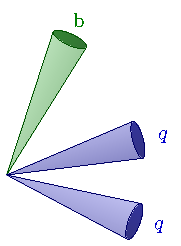
\includegraphics[width=0.28\textwidth]{Feynman/sep.pdf}
    \hfill
    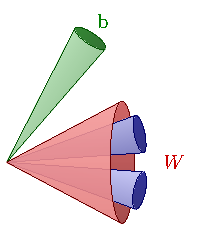
\includegraphics[width=0.28\textwidth]{Feynman/W.pdf}
    \hfill
    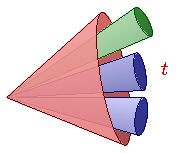
\includegraphics[width=0.28\textwidth]{Feynman/top.pdf}
    \caption{A top quark decay with increasing momentum, showing the transition from three separately resolved jets (left), to a $W$-jet and a $b$-jet (middle), to a single fat jet (right).}
    \label{fig:jet_topologies}
\end{figure}

The number of subjets and the angular separation of these subjets can be used to identify the initiating particle.
One commonly used set of observables to describe jet substructure is its \emph{N-subjettiness}~\cite{Subjet}, denoted by ${\tau_N}$.
N-subjettiness is a measure of how well a jet can be decomposed into $N$ subjets.
For a given $N$ these subjets can be found via some clustering algorithm, such as the exclusive-$k_t$ algorithm~\cite{ExclusiveKT}, and then the $\tau_N$ observable is defined as,
\begin{equation}
    \tau_N = \frac{1}{\pt R} \sum_{i} \pt{_i}
    \min(\Delta R_{1i}, \Delta R_{2i}, \ldots, \Delta R_{Ni}),
\end{equation}
where $k$ runs over the constituents of the jet, and $\Delta R_{ij}$ is the angular separation between the $i$th constituent and the $j$th subjet.
The discriminating variable for jet tagging is often the ratio of these observables, $\tau_{21} = \sfrac{\tau_2}{\tau_1}$, is commonly used to distinguish vector boson jets from QCD jets, and
$\tau_{32} = \sfrac{\tau_3}{\tau_2}$, is used to identify top quark jets.

Other commonly used observables relate to the jet's energy correlation functions~\cite{ECF} and their ratios.
The normalized second and third energy correlation functions are defined as,
\begin{align}
    e_{2}(\beta) & = \sum_{i < j} z_i z_j \Delta R_{ij}^\beta,                                                       \\
    e_{3}(\beta) & = \sum_{i < j < k} z{_i} z{_j} z{_k} \Delta R_{ij}^\beta \Delta R_{ik}^\beta \Delta R_{jk}^\beta,
\end{align}
where $\beta$ is a free parameter that controls the angular weighting of the energy correlation, $z_i$ is the \pt fraction of the jet carried by the $i$th constituent, and the summations are over all constituents of the jet.
Analyses at ATLAS make frequent use of the $\Dtwo$ observable~\cite{ATLASD2} to separate 1-prong and 2-prong jets,
\begin{align}
    \Dtwo(\beta) & = \frac{e_3(\beta)}{e_2(\beta)^3}.
\end{align}
Additionally, the Energy Flow Polynomials~(EFPs)~\cite{EFP} are a set of basis features which are sensitive to the underlying substructure of different jet types.

\subsection{Heavy-Flavour Tagging}
\label{sec:flavour_tagging}

Heavy-flavour tagging, or simply flavour tagging, is the process of identifying jets that contain the decay products of $b$-quarks ($b$-jets) or  $c$-quarks ($c$-jets).
Jets originating from the decay of $u-$, $d-$, $s-$ quarks and gluons are collectively called light-jets.
Identifying jets from either process is known as $b$-tagging or $c$-tagging, respectively.
In ATLAS, $b$-tagging plays a critical role in many analyses, particularly those measuring properties of the Higgs boson or the top quark.
Nearly all top quarks decay rapidly into a $W$-boson and a $b$-quark, and the dominant decay mode of the Higgs boson is to a pair of $b$-quarks.

Unlike the methods to distinguish large-radius jets, which rely on the jet substructure, the main distinguishing feature used in $b$-tagging is the extended lifetime of hadrons containing $b$-quarks.
As discussed in \Cref{sec:electroweak}, the weak interaction CKM matrix is nearly diagonal, thus favouring transitions within the same generation.
However, the $b$-quark is approximately 40 times lighter than the $t$-quark; it can only decay into lighter generations and is thus CKM suppressed.

The $b$-hadrons are quasi-stable bound states between a $b$-quark and one or two lighter quarks.
They have an average lifetime of around $1.5~\ps$~\cite{ParticleDataGroup} and if emitted with $\pt=50~\GeV$ would travel around $L_{xy} = 5~\mm$ in the transverse plane before decaying.
This distance can be resolved by the ID vertex fitting algorithms and would result in a vertex with a notable transverse displacement, as shown in \Cref{fig:btagging}.
The presence of a high mass secondary vertex within a jet is the primary feature used in $b$-tagging.

\begin{figure}[htb]
    \centering
    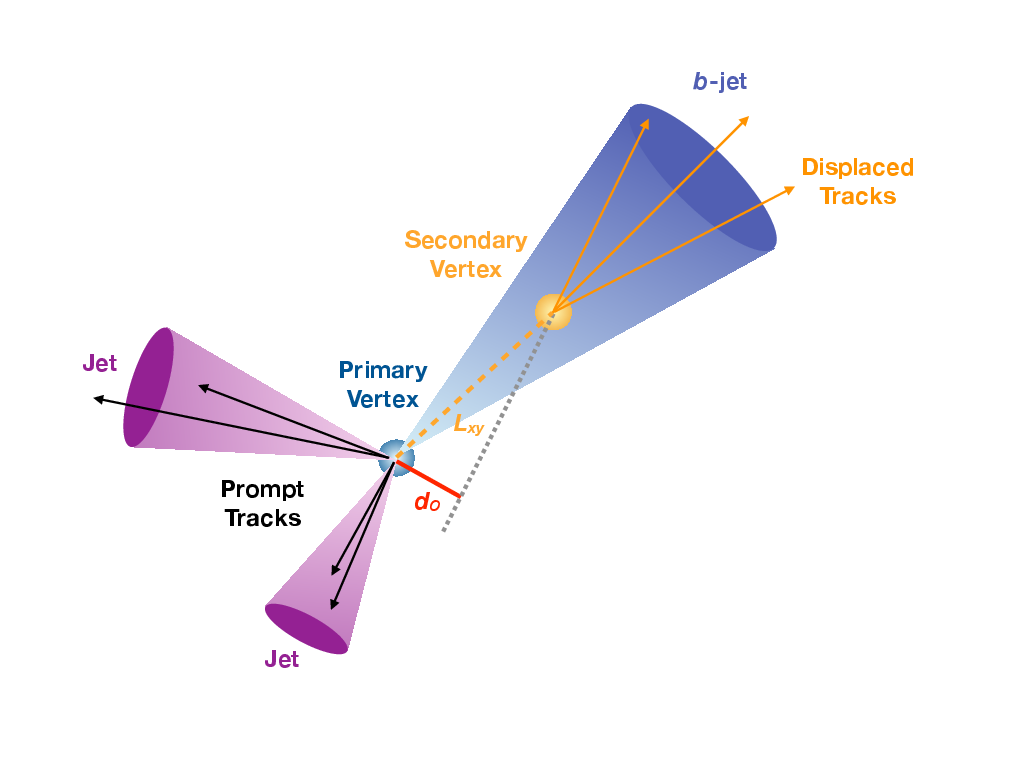
\includegraphics[width=0.75\textwidth]{Figures/cern_atlas/bjet.png}
    \caption{An interaction producing two light-flavour jets and one $b$-jet in the transverse plane. $B$-hadrons have a transverse decay length $L_{xy}$ of a few millimetres, creating displaced tracks and a secondary vertex. The transverse impact parameter (d0) is the closest approach distance of these tracks to the primary vertex, typically large for b-hadrons. Image taken from Ref.~\cite{BJetImage}.}
    \label{fig:btagging}
\end{figure}

Flavour tagging at ATLAS has evolved over many years.
Typically, the tools return the likelihood of a $b$- $c$- or light-jet, given some properties of the associated tracks.
A collection of comparisons between these algorithms used in $b$-tagging is shown in \Cref{fig:btagging_roc}.
Several handcrafted algorithms were designed for flavour tagging before the start of Run 1, such as IPxD~\cite{IPxD}, SV1~\cite{SV1}, and JetFitter~\cite{JetFitter}.
Each tagger used a unique approach to extract different high level features from the jet and associated tracks.
They also yielded different performances depending on the phase space.
It was found that combining the most discriminating features from each in a single neural network resulted in a more versatile tagger known as MV1~\cite{MV1}, which was used at the start of Run 1.
At the start of Run 2, it was replaced by MV2~\cite{MV2}, a boosted decision tree with similar inputs.
In 2017, it was replaced by DL1~\cite{DL1}, a neural network again with much the same approach.
These figures plot the $b$-jet efficiency against light and $c$-jet rejection.

Also introduced at this time was the first tagger based purely on the raw collection of tracks and their parameters, known as RNNIP~\cite{RNNIP}.
This was a recurrent neural network (RNN) that processed all the tracks in the jet sequentially to determine the three class probabilities.
Again, the performance was improved by combining the outputs of RNNIP with the other algorithms (IPxD, SV1, JetFitter), yielding the DL1r tagger~\cite{Run2FTAlgs}.
A second track-based tagger known as DIPS~\cite{DIPS} was developed in 2020.
It used the deep sets architecture~\cite{DeepSets}, and the corresponding combined tagger was labelled DL1d~\cite{AlexThesis}.

The most recent iteration is a departure from the previous approach of combining multiple high level and track based taggers.
In 2022 ATLAS introduced the GN1 tagger~\cite{GN1} which is a graph neural network, \Cref{ch:gnns}, that only uses the track information.
This single network, simultaneously performs jet tagging, as well as vertex matching and track classification trained end-to-end.

More details on the GN1 tagger are provided in \Cref{ch:spice}, which also details the development of a new flavour tagging algorithm, GN2, which would supersede it.

\begin{figure}[h]
    \centering
    \begin{subfigure}{0.435\linewidth}
        \centering
        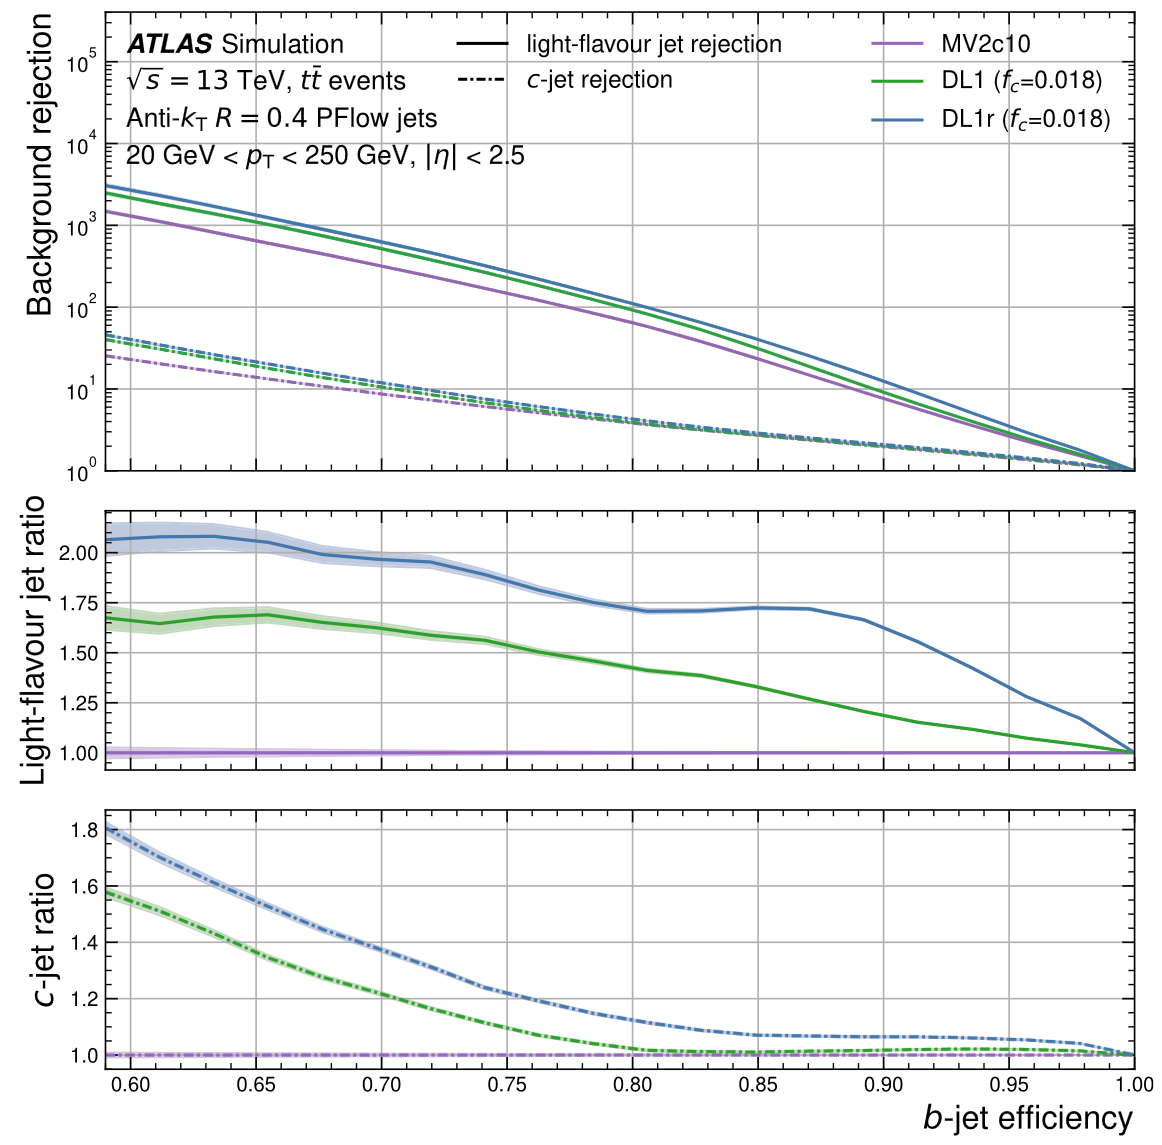
\includegraphics[width=\linewidth]{Figures/cern_atlas/dl1r.png}
        \caption{}
        \label{fig:dl1r}
    \end{subfigure}
    \begin{subfigure}{0.555\linewidth}
        \centering
        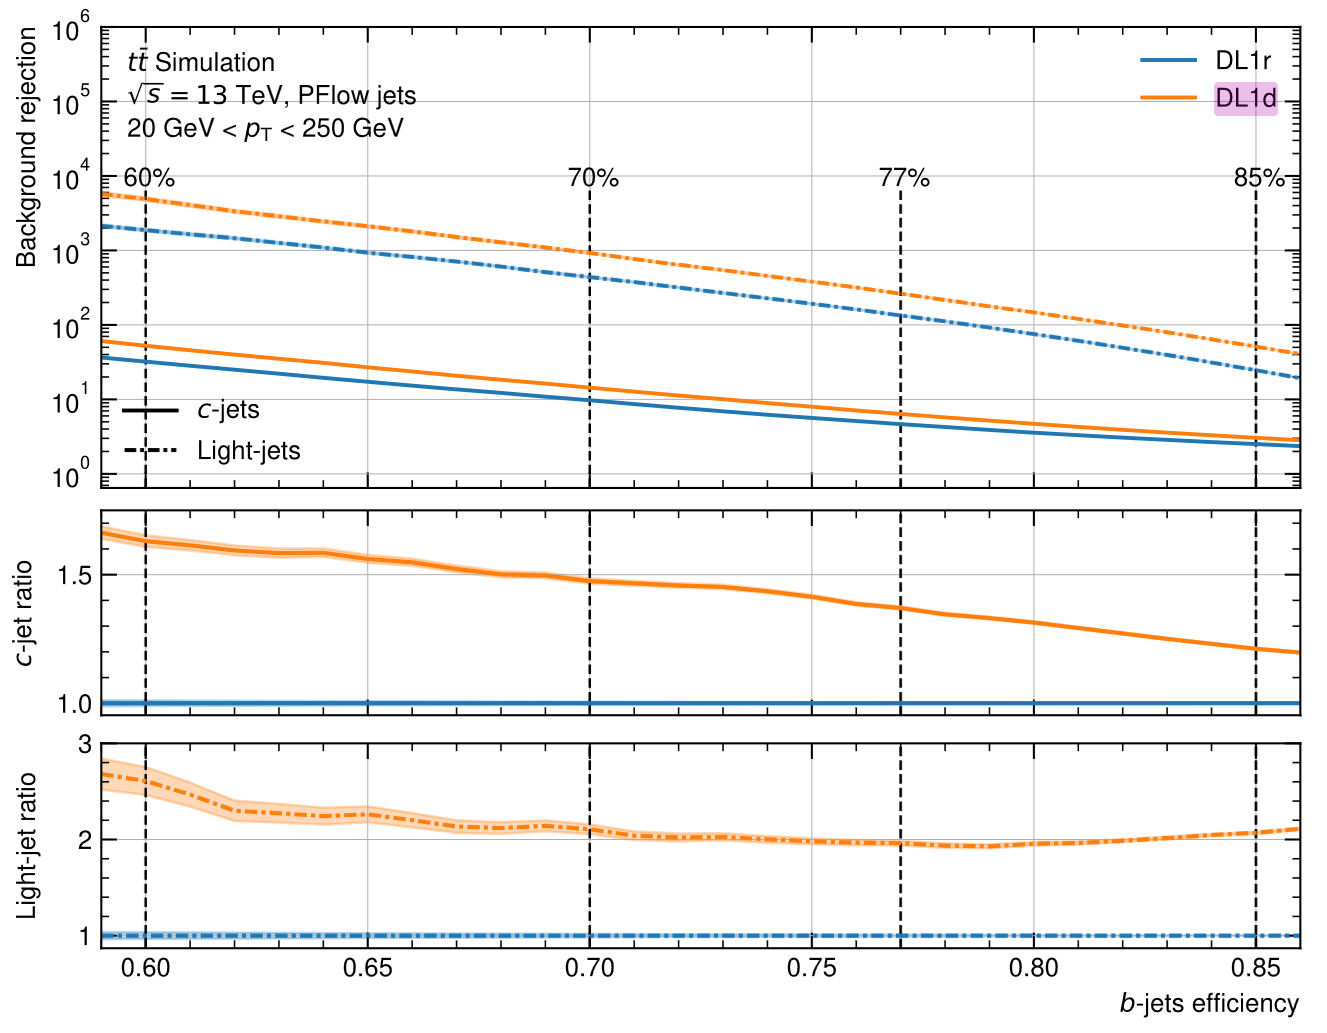
\includegraphics[width=\linewidth]{Figures/cern_atlas/dl1d.png}
        \caption{}
        \label{fig:dl1d}
    \end{subfigure}
    \begin{subfigure}{0.85\linewidth}
        \centering
        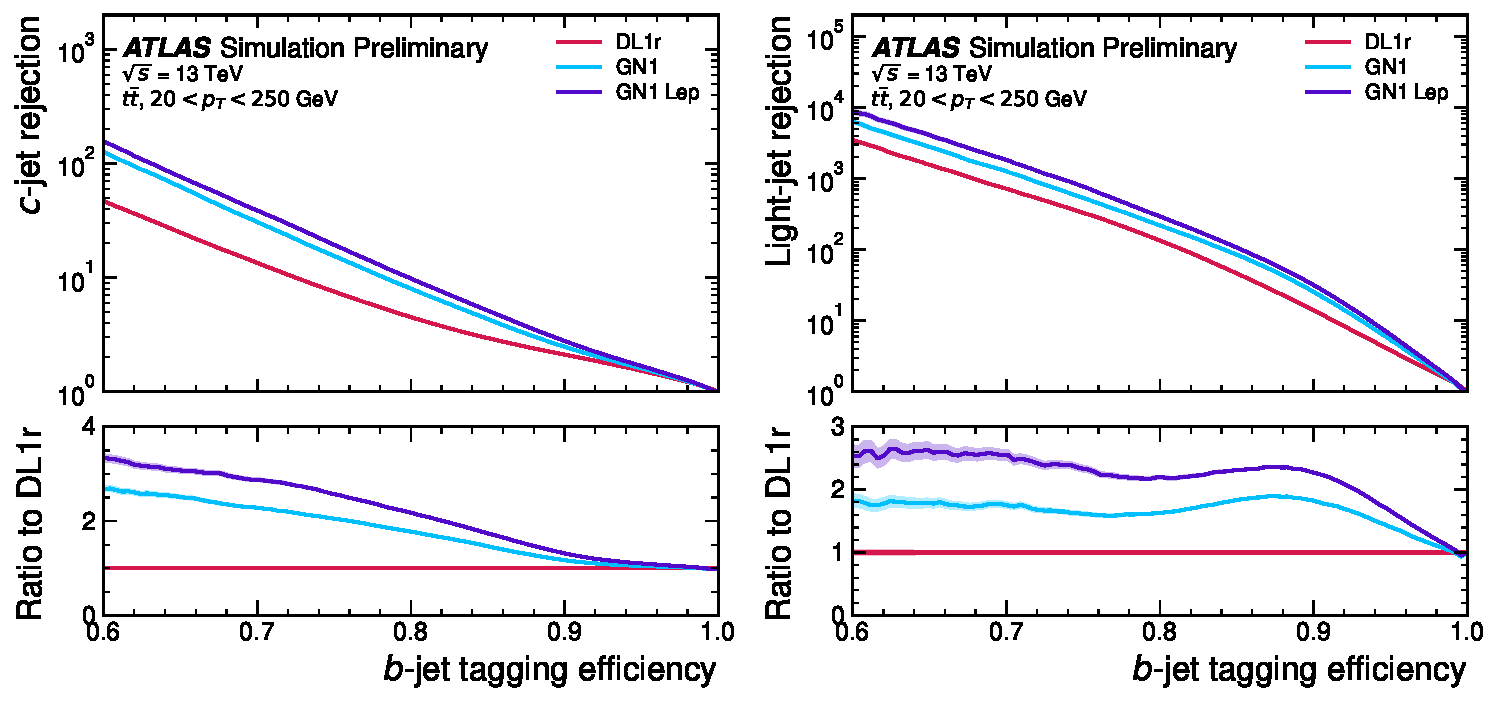
\includegraphics[width=\linewidth]{Figures/cern_atlas/gn1roc.pdf}
        \caption{}
        \label{fig:gn1r}
    \end{subfigure}
    \caption{The rejection factors for light-jets and c-jets as a function of the $b$-tagging efficiency for the different algorithms used by ATLAS over the years as measured on simulated \ttbar datasets. \subref{fig:dl1r} shows the performance of the MV2, DL1, DL1r taggers with the bottom panels showing the performance ratio to MV2. \subref{fig:dl1d} shows the performance of the DL1d and DL1r taggers with the bottom panels showing the performance ratio to DL1r. \subref{fig:gn1r} shows the performance of the GN1 tagger. Images taken from Refs.~\cite{Run2FTAlgs,AlexThesis,GN1} respectively.
    }
    \label{fig:btagging_roc}
\end{figure}
